\def\year{2020}\relax
%File: formatting-instruction.tex
\documentclass[letterpaper]{article} % DO NOT CHANGE THIS
\usepackage{aaai20}  % DO NOT CHANGE THIS
\usepackage{times}  % DO NOT CHANGE THIS
\usepackage{helvet} % DO NOT CHANGE THIS
\usepackage{courier}  % DO NOT CHANGE THIS
\usepackage[hyphens]{url}  % DO NOT CHANGE THIS
\usepackage{graphicx} % DO NOT CHANGE THIS
\urlstyle{rm} % DO NOT CHANGE THIS
\def\UrlFont{\rm}  % DO NOT CHANGE THIS
\usepackage{graphicx}  % DO NOT CHANGE THIS
\frenchspacing  % DO NOT CHANGE THIS
\setlength{\pdfpagewidth}{8.5in}  % DO NOT CHANGE THIS
\setlength{\pdfpageheight}{11in}  % DO NOT CHANGE THIS
\usepackage[UTF8]{ctex}
\usepackage{booktabs} %table topline,midline,bottomline
\usepackage{algorithm}
\usepackage{algorithmicx}
%\nocopyright
%PDF Info Is REQUIRED.
% For /Author, add all authors within the parentheses, separated by commas. No accents or commands.
% For /Title, add Title in Mixed Case. No accents or commands. Retain the parentheses.
 \pdfinfo{
/Title (Synthesis of Registered Multimodal MRI with Lesion Label)
/Author (Yili Qu,Wanqi Su,Chufu Deng,Ying Wang,Yutong Lu,Nong Xiao,Zhiguang Chen)
} %Leave this	
% /Title ()
% Put your actual complete title (no codes, scripts, shortcuts, or LaTeX commands) within the parentheses in mixed case
% Leave the space between \Title and the beginning parenthesis alone
% /Author ()
% Put your actual complete list of authors (no codes, scripts, shortcuts, or LaTeX commands) within the parentheses in mixed case. 
% Each author should be only by a comma. If the name contains accents, remove them. If there are any LaTeX commands, 
% remove them. 

% DISALLOWED PACKAGES
% \usepackage{authblk} -- This package is specifically forbidden
% \usepackage{balance} -- This package is specifically forbidden
% \usepackage{caption} -- This package is specifically forbidden
% \usepackage{color (if used in text)
% \usepackage{CJK} -- This package is specifically forbidden
% \usepackage{float} -- This package is specifically forbidden
% \usepackage{flushend} -- This package is specifically forbidden
% \usepackage{fontenc} -- This package is specifically forbidden
% \usepackage{fullpage} -- This package is specifically forbidden
% \usepackage{geometry} -- This package is specifically forbidden
% \usepackage{grffile} -- This package is specifically forbidden
% \usepackage{hyperref} -- This package is specifically forbidden
% \usepackage{navigator} -- This package is specifically forbidden
% (or any other package that embeds links such as navigator or hyperref)
% \indentfirst} -- This package is specifically forbidden
% \layout} -- This package is specifically forbidden
% \multicol} -- This package is specifically forbidden
% \nameref} -- This package is specifically forbidden
% \natbib} -- This package is specifically forbidden -- use the following workaround:
% \usepackage{savetrees} -- This package is specifically forbidden
% \usepackage{setspace} -- This package is specifically forbidden
% \usepackage{stfloats} -- This package is specifically forbidden
% \usepackage{tabu} -- This package is specifically forbidden
% \usepackage{titlesec} -- This package is specifically forbidden
% \usepackage{tocbibind} -- This package is specifically forbidden
% \usepackage{ulem} -- This package is specifically forbidden
% \usepackage{wrapfig} -- This package is specifically forbidden
% DISALLOWED COMMANDS
% \nocopyright -- Your paper will not be published if you use this command
% \addtolength -- This command may not be used
% \balance -- This command may not be used
% \baselinestretch -- Your paper will not be published if you use this command
% \clearpage -- No page breaks of any kind may be used for the final version of your paper
% \columnsep -- This command may not be used
% \newpage -- No page breaks of any kind may be used for the final version of your paper
% \pagebreak -- No page breaks of any kind may be used for the final version of your paperr
% \pagestyle -- This command may not be used
% \tiny -- This is not an acceptable font size.
% \vspace{- -- No negative value may be used in proximity of a caption, figure, table, section, subsection, subsubsection, or reference
% \vskip{- -- No negative value may be used to alter spacing above or below a caption, figure, table, section, subsection, subsubsection, or reference

\setcounter{secnumdepth}{2} %May be changed to 1 or 2 if section numbers are desired.

% The file aaai20.sty is the style file for AAAI Press 
% proceedings, working notes, and technical reports.
%
\setlength\titlebox{2.5in} % If your paper contains an overfull \vbox too high warning at the beginning of the document, use this
% command to correct it. You may not alter the value below 2.5 in
\title{基于条件生成对抗网络的配准多模态脑MRI合成Synthesis of Registered Multimodal MRI with Lesion Label }
%Your title must be in mixed case, not sentence case. 
% That means all verbs (including short verbs like be, is, using,and go), 
% nouns, adverbs, adjectives should be capitalized, including both words in hyphenated terms, while
% articles, conjunctions, and prepositions are lower case unless they
% directly follow a colon or long dash
\author{\Large \textbf{Yili Qu,Wanqi Su,Chufu Deng,}\\ \Large \textbf{Ying Wang,Yutong Lu,Nong Xiao,Zhiguang Chen}\\  % All authors must be in the same font size and format. Use \Large and \textbf to achieve this result when breaking a line
 %If you have multiple authors and multiple affiliations
% use superscripts in text and roman font to identify them. For example, Sunil Issar,\textsuperscript{\rm 2} J. Scott Penberthy\textsuperscript{\rm 3} George Ferguson,\textsuperscript{\rm 4} Hans Guesgen\textsuperscript{\rm 5}. Note that the comma should be placed BEFORE the superscript for optimum readability
School of Data and Computer Science\\ Sun Yet-Sen University\\	
quyli@mail2.sysu.edu.cn% email address must be in roman text type, not monospace or sans serif
}
\begin{document}

\maketitle

\begin{abstract}
在基于大量数据驱动的医学影像智能处理任务中,医学影像数据的收集和采集是非常困难的,尤其是配准的多模态医学影像数据。合成的医学影像数据可以很好地缓解数据不足的问题。我们基于无监督的条件生成对抗网络模型实现了完全从随机噪声生成配准的多模态医学影像,并且可以根据自由选定的病灶标签有效地生成对应的病灶信息。我们在BRATS2015上进行了多项验证实验,验证了我们的合成MRI可以在医学影像智能处理任务中作为预训练数据或增强数据使用,并能大幅度提高模型的泛化能力。
In a large number of data-driven medical image intelligent processing tasks, the collection and acquisition of medical image data is very difficult, especially the registered multimodal medical image data. Synthetic medical image data can well alleviate the problem of insufficient data. In this paper, based on the unsupervised CGAN model, we achieve the generation of registered multimodal medical images from random noise and corresponding lesion information can be efficiently generated based on the freely selected lesion label. We conducted a number of validation experiments on BRATS2015 to verify that our synthetic MRI can be used as pre-trained data or enhanced data in medical image intelligent processing tasks, and can greatly improve the generalization ability of the model.
\end{abstract}
	
\section{Introduction}
核磁共振成像(MRI)是一种常见的医学影像,根据成像参数的不同可以有多种模态,例如T1、T2、T1c等。不同的模态对医生具有不同的参考价值,医生往往需要多个模态的影像互相对照才能做出准确的判断。在医学影像的智能处理任务的训练和学习中,我们往往也期望获得更多模态的影像,例如采用卷积神经网络(CNN)\cite{86krizhevsky2012imagenet}或生成对抗网络(GAN)\cite{25goodfellow2014generative}进行的医学图像处理任务。
Magnetic resonance imaging (MRI) is a common medical image that can have multiple modalities depending on imaging parameters, such as T1, T2, T1c and so on. Different modalities have different reference values for doctors. To make accurate judgments, doctors often need multiple modal images to compare with each other. In the training and learning of medical image intelligent processing tasks, we often expect to obtain more modal images, such as medical image processing tasks based on Convolutional Neural Networks (CNN)\cite{86krizhevsky2012imagenet} or Generative Adversarial Networks (GAN)\cite{25goodfellow2014generative}. 

当同一个病人的同一个部位通过不同的成像技术得到不同的模态时,如果成像位置和视角是一致的,那么得到的不同模态的影像就是对齐的,我们称之为这些模态之间是配准的。相较于单模态数据,配准的多模态影像数据能提供更多的信息,可以支撑更多和更复杂的应用场景,满足深度神经网络对训练数据的需求,有助于提供更加高效可靠的智能诊断服务。对于医生来说,获取不同模态的影像需要花费更长的时间并且需要患者的耐心配合。对于医学影像智能处理任务的研究者来说,多模态的MRI数据集十分稀缺,收集难度非常大,尤其是罕见病数据,而配准的数据则更加稀少,这使得很多的训练任务无法实现。因此,通过应用图像合成技术扩展数据集,从已有的单模态图像转换为配准的多模态图像、从随机噪声生成配准的多模态医学影像,有着广泛的用途和深远的意义。
When obtaining different modalities from the same part of the same patient  through different imaging techniques, these modalities are considered to be registered if the imaging position and the viewing angle are identical.  Compared with unimodal data, the registered multimodal image data can provide more information, can support more complex application scenarios, meet the training data requirements of deep neural networks, and help to provide  intelligent diagnostic services more efficient and more reliable. For doctors, it takes longer to acquire images of different modalities and requires patient patience. For researchers of medical image intelligent processing tasks, multimodal MRI datasets are scarce, and the collection is very difficult, especially rare disease data, and the registered data is even rarer, which makes many training tasks impossible. Therefore, the application of image synthesis technology to extend datasets, translate existing unimodal images to registered multimodal images, generate registered multimodal images from random noise, has a wide range of uses and far-reaching significance.

在GAN之前,一些研究使用图字典映射\cite{22burgos2015robust}、稀疏编码\cite{33huang2017simultaneous},\cite{34vemulapalli2015unsupervised},CNN\cite{36vannguyen2015crossdomain}等探索了医学影像的跨模态转换。此后许多研究使用GAN能产生更高质量的转换结果\cite{1zhao2018modular},\cite{5liang2018generative},\cite{6zhu2017unpaired},\cite{13choi2018stargan:}。得益于GAN的强大能力,目前,采用GAN实现跨模态医学影像转换成为主流\cite{2zhang2018translating},\cite{20nie2017medical},\cite{35osokin2017gans},\cite{36vannguyen2015crossdomain},\cite{40kamnitsas2017unsupervised}。一般的转换基于成对的数据,最近也有研究从不成对的跨域数据中学习\cite{2zhang2018translating}。最近的研究有将像素到像素的GAN应用于脑部MRI到CT图像的转换\cite{20nie2017medical},\cite{40kamnitsas2017unsupervised}、视网膜血管注释到图像的转换\cite{41costa2017towards}、基于CycleGAN\cite{6zhu2017unpaired}的心脏MRI到CT图像的相互转换与分割\cite{20nie2017medical}等。对于多模态的合成,\cite{84chartsias2018multimodal}实现多输入多输出的MRI合成,但对输入的多模态数据要求配准。基于此,\cite{85joyce2017robust}改进实现存在缺失或未配准的多输入合成模型,能够从其输入的任何子集执行MRI图像合成,但限制了输出为单一模态,且模型不可扩展。\cite{66miao2018dilated}针对医学图像配准进行了深入研究。\cite{4shin2018medical}应用GAN合成脑肿瘤图像实现数据增强和数据匿名化,但需要额外训练解剖结构分割网络,且要求数据集带有病灶分割标签,模型泛化能力弱。\cite{41costa2017towards}研究了基于变分自编码器(VAE)\cite{87kingma2014auto-encoding},\cite{88rezende2014stochastic}的思想实现血管注释图的随机生成,进而合成彩色视网膜图像。在当前的这些医学影像合成的研究中,大多仅探索了两个不同模态之间的转换合成\cite{2zhang2018translating},\cite{20nie2017medical},\cite{22burgos2015robust},\cite{34vemulapalli2015unsupervised},\cite{35osokin2017gans},\cite{36vannguyen2015crossdomain},\cite{40kamnitsas2017unsupervised},对多模态的研究还很稀少\cite{84chartsias2018multimodal},\cite{85joyce2017robust},\cite{4shin2018medical},而在医学影像处理领域之外,多域转换的发展最近已经有了进展\cite{1zhao2018modular},\cite{5liang2018generative},\cite{13choi2018stargan:},\cite{27isola2017image-to-image}。

Some studies explored cross-modal medical images translation prior to GAN by using graph dictionary mapping\cite{22burgos2015robust}, sparse coding\cite{33huang2017simultaneous},\cite{34vemulapalli2015unsupervised}, and CNN\cite{36vannguyen2015crossdomain}. Since then, many studies used GAN to generate higher quality translation results\cite{1zhao2018modular},\cite{5liang2018generative},\cite{6zhu2017unpaired},\cite{13choi2018stargan:}. Owe to the powerful capabilities of GAN, it has become the mainstream to achieve multimodal medical image translation\cite{2zhang2018translating},\cite{20nie2017medical},\cite{35osokin2017gans},\cite{36vannguyen2015crossdomain},\cite{40kamnitsas2017unsupervised}. The general translation is based on paired data, some studies have also learned from unpaired cross-modal data\cite{2zhang2018translating}. Recent studies have realized brain MRI to CT image translation with pixel-to-pixel GAN\cite{20nie2017medical},\cite{40kamnitsas2017unsupervised}, retinal vascular annotation to image translation\cite{41costa2017towards}, CycleGAN-based\cite{6zhu2017unpaired} cardiac MRI to CT image translation and segmentation\cite{20nie2017medical}. For multimodal synthesis, \cite{84chartsias2018multimodal} implements MRI synthesis of multiple inputs multiple outputs, but requires registration for input multimodal data. Based on this, \cite{85joyce2017robust} improves and implements a missing or unregistered multi-input synthesis model that can perform MRI image synthesis from any subset of its inputs, but limits the output to a single modality and the model is not scalable. \cite{66miao2018dilated} has conducted in-depth research on medical image registration. \cite{4shin2018medical} applys GAN to synthesize brain tumor images for data enhancement and data anonymization, but additional training of anatomical segmentation networks is required, and the dataset is required to have lesion segmentation labels, so the model generalization ability is weak. \cite{41costa2017towards} studies the random generation of vascular annotation maps based on the idea of Variational Auto-Encoder (VAE)\cite{87kingma2014auto-encoding, 88rezende2014stochastic}, and then synthesizes color retinal images. In these current studies of medical image synthesis, most are two-modal translation\cite{2zhang2018translating},\cite{20nie2017medical},\cite{22burgos2015robust},\cite{34vemulapalli2015unsupervised},\cite{35osokin2017gans},\cite{36vannguyen2015crossdomain},\cite{40kamnitsas2017unsupervised}, and the study of multimodal translation is very rare\cite{84chartsias2018multimodal},\cite{85joyce2017robust},\cite{4shin2018medical}. Outside the field of medical image processing, the development of many-to-many translation has recently made progress\cite{1zhao2018modular},\cite{5liang2018generative},\cite{13choi2018stargan:},\cite{27isola2017image-to-image}.

目前针对医学影像合成的研究存在模态数量难以扩展、需要配准训练数据、依赖于复杂的大型网络、无法添加或保留病灶、无法从随机矩阵开始生成、需要额外的训练数据等各项问题,且大多数研究对合成数据的评价依赖于经验医师的人工视觉效果评估,没有进行客观的量化检验。因此,我们设计了一种基于条件生成对抗网络(CGAN)\cite{70mirza2014conditional}的配准多模态MRI生成的方法,采用无监督学习方法,训练数据无需配准,输入随机正态分布矩阵进而生成一组有病灶标签的多模态配准MRI。我们在BRATS2015数据集上进行了带肿瘤分割标签的脑多模态MRI生成实验,并验证了我们的合成数据中病灶信息的有效程度和合成数据在肿瘤病灶分割实验中的可用程度。我们将开源我们的代码。总的来说,我们的工作主要体现在以下三个方面:
At present, there are various problems in the research of medical image synthesis, such as the difficulty of expanding the number of modalities, the need to registered training data, relying on complex large networks, the inability to add or retain lesions, the inability to generate from random matrices, and the need of additional training data, etc. Moreover, the evaluation of synthetic data in most studies relies on the evaluation of artificial visual effects by experienced physicians, without objective quantitative evaluation. Therefore, we design a registered multimodal MRI generation scheme based on the Conditional Generative Adversarial Networks (CGAN)\cite{70mirza2014conditional}. With unsupervised learning method, training data do not need to be registered. Our solution can receive a random normal distribution as input to generate a set of labeled multimodal registration MRI. We perform multimodal brain MRI generation experiments with tumor segmentation labels on BRATS2015, and verify the effectiveness of lesion information and the availability of synthetic data in tumor lesion segmentation experiments. See the open source code for details. Specifically, our contribution is in the following three areas:

\begin{itemize}
	\item \textbf{结构特征图的提取与随机生成Extraction and Random Generation of Structural Feature Maps}
	我们针对脑MRI提出了一种解剖结构特征的提取方法,无需额外的解剖结构分割标签或标签提取训练,可直接从任意模态的真实影像提取得到结构特征,用以辅助GAN学习生成更合理的合成影像。我们训练了一个结构特征图生成器实现了从多维正态分布生成结构特征图。我们的提取方法可以直接获取真实影像的解剖结构特征,在提升合成影像质量同时不带来额外参数、计算开销小,而随机生成方法可以无限地生成丰富多样的结构特征图。
	We propose an extraction method for anatomical features for medical images. Without additional anatomical segmentation labels or label extraction training, structural feature maps can be extracted directly from real images of arbitrary modalities ,and assist GAN to learn to generate more reasonable synthetic images. The extraction method can directly obtain the anatomical features of real images, and improve the quality of synthetic images without introducing additional parameters and computation overhead. We also train a structural feature map generator to generate structural feature maps from multidimensional normal distribution. The random generation method can generate rich and diverse structural feature maps indefinitely.
	\item \textbf{带标签多模态配准影像的合成Synthesis of Registered Multimodal MRI with Lesion Label}
	我们使用随机生成的结构特征图,融合随机的病灶标签,通过生成器合成配准的多模态MRI。我们探讨了多种病灶生成指导方法,并通过病灶生成指导方法实现了在多模态MRI的合成过程中根据输入病灶标签有效地生成对应的病灶信息。在训练时我们无需配准的数据,除病灶标签外无需额外的标签数据,而合成的数据是配准的,输入的随机病灶标签即为合成数据的病灶标签。我们的方法能够便捷快速地构建带标签的配准多模态MRI数据集。
	We use randomly generated structural feature maps to fuse with random lesion labels and then synthesize the registered multimodal MRIs through the generator. We explore a variety of lesion generation guidance methods to achieve effective mapping of lesions based on input lesion labels during multimodal MRI synthesis. In training, no registration data is required, no additional label data is required except for the lesion label, the synthetic data is registered, and the random lesion label is the lesion label of the synthetic data. Our solution enables fast and easy construction of registered multimodal MRI datasets with label.
	\item \textbf{合成数据可用性的客观验证方法Objective Verification Method for Synthetic Data Availability}
	我们使用不同数据量的合成数据和真实数据构建的数据集来训练病灶分割网络,验证了合成数据可以在医学影像智能处理任务可以作为预训练数据和增强数据来提高模型的泛化能力从而提高分割精度。对比传统合成影像质量的主观评价方法,我们更加客观地呈现了合成数据在智能病灶处理任务中的可用性。
	We construct datasets with different amount of synthetic and real data to train the lesion segmentor, and verify that the synthetic data can be used as pre-training data and enhanced data in the medical image intelligent processing tasks to improve the generalization ability of the model and improve the segmentation precision. Compared with the traditional subjective evaluation method of synthetic image quality, we present the availability of synthetic data in intelligent lesion processing tasks more objectively.
\end{itemize}


\section{方法Method}
\label{method}
我们在多模态脑MRI的合成任务上展示我们的方法。在本文的实例中,我们合成的病灶为肿瘤,病灶标签为肿瘤分割标签,病灶处理任务为病灶分割。我们的方法对合成部位、病灶类型、病灶处理任务、具体的模态和模态数量等不做限制,通过下述实例的展示,我们能很容易的将该方法推广应用到其他的类似任务。
We perform our scheme on multimodal brain MRI synthesis task, in which the synthetic lesion is tumors, the lesion label is a tumor segmentation label, and the lesion processing task is lesion segmentation. Our scheme does not limit the synthesis of human parts, lesion types, lesion processing tasks, specific modality and the number of modalities. We can easily apply this method to other similar tasks through the following example.
\subsection{整体架构Overall Architecture}
\begin{figure}[t]
	\centering
	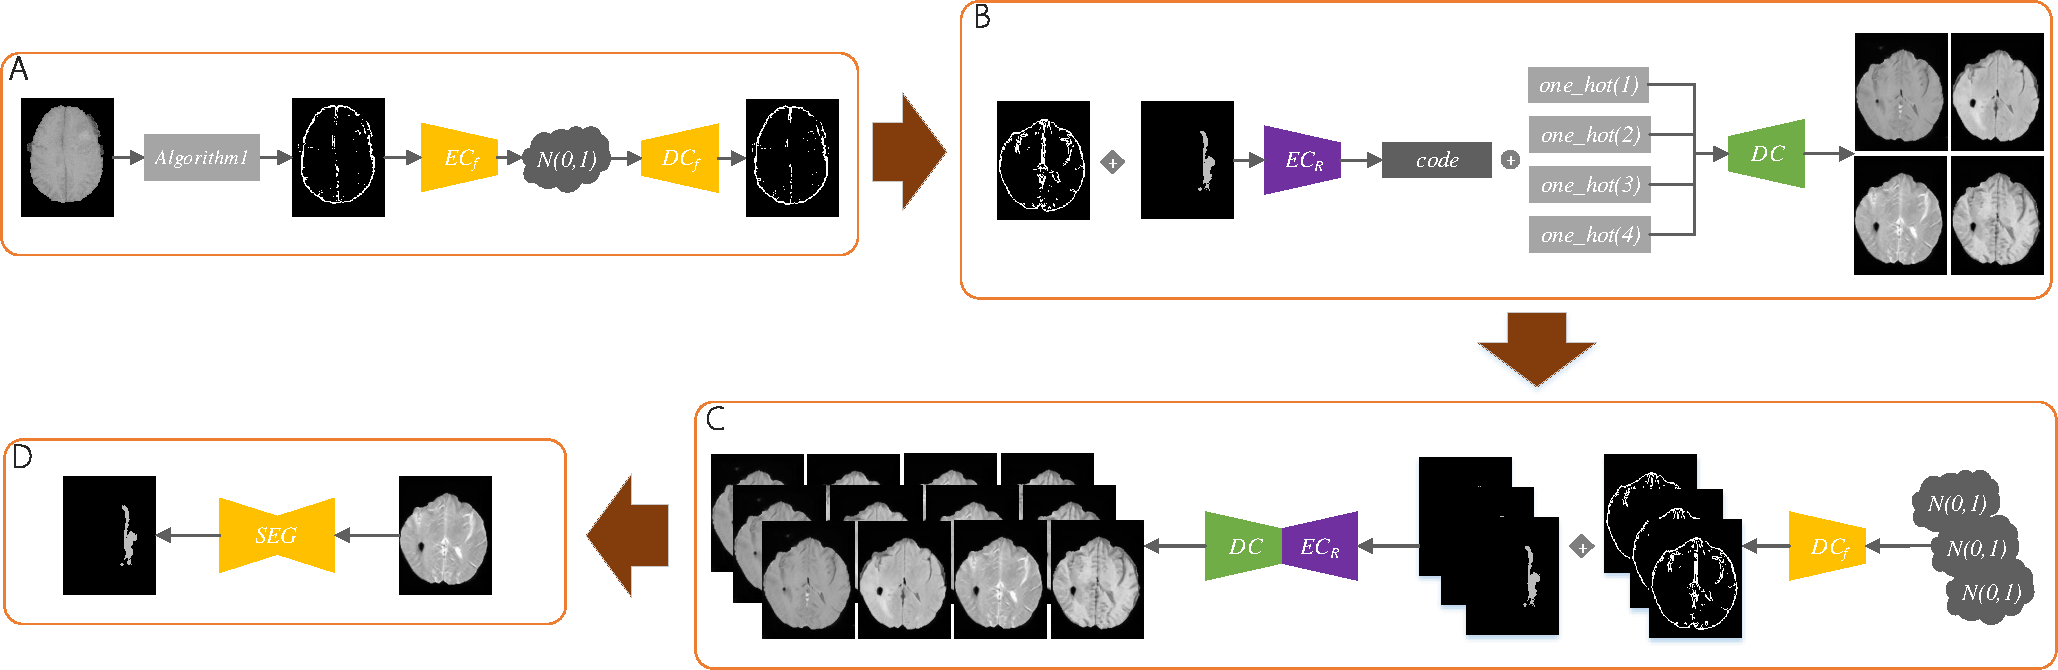
\includegraphics[width=0.98\columnwidth]{figures/architecture}
	\caption{整体架构图.Overall Architecture.}
	\label{architecture}
\end{figure}
如图~\ref{architecture}所示,我们的方案包括结构特征图提取和生成、多模态MRI生成、构建合成数据集、合成数据可用性验证四个主要阶段。
As shown in Fig.~\ref{architecture}, our scheme includes four main stages: structural feature map extraction and random generation, multimodal MRI generation, construction of synthetic datasets, and synthetic data availability verification.

结构特征图提取和生成阶段我们将获得一个结构特征图生成器,能从随机的正态分布矩阵生成结构特征图。该阶段我们训练的模型模包括一个结构特征图编码器、一个结构特征图解码器、一个结构特征图鉴别器、一个编码分布鉴别器和一个结构特征图掩膜生成器。
In the structural feature map extraction and random generation stage, we will obtain a structural feature map generator that can generate structural feature maps from the random normal distribution matrix. Models we train at this stage includes a structural feature map encoder, a structural feature map decoder, a structural feature map discriminator, a code distribution discriminator and a structural feature mask generator.

多模态MRI生成阶段我们产出一个条件生成器,其以结构特征图为输入,能根据不同的独热条件向量生成不同模态的MRI,并且可在结构特征图上添加病灶标签使得生成的MRI具有对应的病灶信息。该阶段我们训练的模型模块包括一个结构特征图与病灶标签的融合图编码器、不同模态的病灶分割器、一个MRI编码器、一个MRI解码器、一个MRI鉴别器和一个MRI编码鉴别器。
In the multimodal MRI generation stage, we generate a conditional generator with input of structural feature maps, which can generate MRIs of different modalities according to different one-hot conditional vectors, and can add lesion labels on the structural feature maps to generate MRI has corresponding lesion information. At this stage, we train a structural feature map and lesion label fusion encoder, a lesion segmentor for each modality, an MRI encoder, an MRI decoder, an MRI discriminator and an MRI code discriminator.

在构建合成数据集阶段,我们使用前两个阶段产出的模型先从随机正态分布矩阵生成足量的结构特征图,再与随机病灶标签进行信息融合,最后通过条件生成器生成配准的多模态MRI,从而构建出一个合成数据集。
In the stage of constructing the synthetic datasets, we use the model produced in the first two stages to generate a sufficient number of structural feature maps from the random normal distribution matrix and then randomly fuse with real lesion labels, and finally generate the registered multimodal MRI to construct synthetic datasets.

在合成数据可用性验证阶段,我们首先根据真实的数据为每个MRI模态单独训练一个病灶分割器,并在真实数据集中进行分割能力测试,再用该分割器对采用不同的病灶生成组件来指导病灶生成的合成数据进行分割测试。然后,我们使用由不同数据量的合成数据和真实数据构建的数据集来对病灶分割网络进行训练,训练充分后再在真实测试数据集上进行分割测试,对比各项测试结果,以验证合成数据在肿瘤病灶分割训练中的可用性。
In the synthetic data availability verification stage, we train a lesion segmentor for each MRI modality based on real data, and perform segmentation ability tests on real dataset. Then these segmentors are used to perform segmentation tests on the synthetic data generated by different lesion generation guidance methods. In addition, we use datasets constructed from synthetic data and real data of different amounts to train the lesion segmentor. After training, the segmentation ability test is performed on the real dataset, and the test results are compared to verify the availability of the synthetic data in lesion segmentor training.

\subsection{结构特征图提取方法Structural Feature Map Extraction Method}

直接从随机噪声通过生成对抗训练生成的医学影像通常训练困难且难以生成真实的结构信息。我们将医学影像中提供基本轮廓和结构信息的图像称为其结构特征图,例如视网膜血管分布图可视为视网膜图像的结构特征图\cite{41costa2017towards}。结构特征图可以为医学影像的合成提供必要的基础指导信息,例如合成脑部MRI图像时一些研究从脑分割标签图获取基本的结构信息\cite{4shin2018medical}。然而,视网膜血管分布图和脑分割标签图等常用的结构特征图都需要额外的数据和训练才能实现从原图提取出结构特征图。为此,我们首先设计了下述直接从脑MRI提取结构特征图的方法,该方法具有运算快、无需训练、无需额外数据等优点。
Medical images generated directly from random noise by GAN are often difficult to train and difficult to generate real structural information. We call image that provide basic contour and structure information as structural feature map. For example, a retinal blood vessel distribution map can be regarded as a structural feature map of a retinal image\cite{41costa2017towards}. Structural feature maps can provide necessary basic guidance for the synthesis of medical images. For example, when synthesizing brain MRI, some studies obtain basic structural information from the brain segmentation label\cite{4shin2018medical}. However, common structural features such as retinal vascular maps and brain segmentation labels require additional data and training to extract structural features from the original image. To this end, we first design a method for extracting structural feature maps directly from brain MRI, which has the advantages of fast operation, no training, no additional data. 

在传统的数字图像处理方法中,Roberts算子\cite{87Roberts}、Prewitt算子\cite{88prewitt}、Sobel算子\cite{89Sobel}等是十分优秀的边缘检测算子,其中Sobel算子常用于脑部医学图像的处理,其卷积核参数和计算公式如图所示。我们探索出了从Sobel算子生成的边缘检测图中进一步提取结构特征的方法,如算法~\ref{alg:1}所示。
In the traditional digital image processing methods, Roberts operator, Prewitt operator, Sobel operator, etc. are excellent edge detection operators. Sobel operator is often used in processing of brain medical images, and their convolution kernel parameters and calculation formula are as shown. As shown in Algorithm~\ref{alg:1}, We explore a method for further extracting structural feature maps from the edge detection maps generated by Sobel operator.
\begin{algorithm}
	\caption{Structural Feature Extraction}
	\label{alg:1}
	\begin{algorithmic}[1]
		\State Input a real image $x$,$beta$ is pixel threshold
		\State $f1 = reduce\_min(sobel(x))$
		\State $f2 = reduce\_max(sobel(x))$
		\State $f1 = mean(f1) - f1$
		\State $f2 = f2 - mean(f2)$
		\State $f1 = ones * (f1 > beta)$
		\State $f2 = ones * (f2 > beta)$
		\State $f = f1 + f2$
		\State $f = ones * (f > 0.)$
	\end{algorithmic}  
\end{algorithm}

在算法~\ref{alg:1}中,我们对一张真实图像用Sobel算子提取得到其横向和纵向的边缘检测图,对两张边缘检测图进行最大值规约和最小值规约得到两张新的边缘检测融合图,然后两张边缘检测融合图分别与各自的平均像素值求差,再对两张差值图根据设定像素阈值进行二值化处理,两张二值图求和后再进行完全的二值化,最后得到的就是我们需要的结构特征图。
In Algorithm~\ref{alg:1} we use Sobel operator to extract the horizontal and vertical edge detection maps from a real image, each perform reduce maximum and reduce minimum to obtain two edge detection fusion maps, each fusion map calculate the difference with average pixel value, the two difference maps are binarized according to the set pixel threshold, and the two binary images are summed and then completely binarized. The final result is the structural feature map we need.

\subsection{随机结构特征图的生成训练Training of Random Structural Feature Map Generation}

在生成结构特征图时,\cite{4shin2018medical}仍然需要真实的MRI作为输入来得到生成的结构特征图,这大大降低了生成数据的多样性,\cite{41costa2017towards}实现了一种从多维正态分布生成视网膜血管分布图的方法,在其基础上,我们设计了一种从随机噪声生成脑部结构特征图的方法,无需额外数据且具有更好的多样性。具体来说,我们结合了变分自编码器与生成对抗网络的特点设计了一种混合网络。首先,我们从真实影像提取得到结构特征图,再通过VAE的编码器将其编码为一个均值矩阵和一个方差矩阵,再与一个随机正态分布矩阵融合为一个近似正态分布矩阵,通过损失约束其逐渐逼近标准正态分布。然后,我们再用VAE的解码器实现从该近似正态分布重建生成结构特征图。解码器通过结构特征图的自监督重建损失进行训练。对于近似正态分布矩阵的损失约束,我们没有采用VAE原本的编码器损失,而是通过一个编码分布鉴别器为编码器提供对抗性损失,此编码分布鉴别器以正态分布矩阵为正样本、输入解码器的近似正态分布矩阵为负样本进行学习。此外,我们还通过$L2$正则损失指导均值矩阵的均值逼近0值,标准差矩阵的均值逼近1值。同时,我们用另一个鉴别器对从真实MRI提取的结构特征图和随机生成的结构特征图进行鉴别学习,并为解码器提供对抗性损失,使得从随机正态分布解码生成的结构特征图越来越逼真。
When generating the structural feature map, \cite{4shin2018medical} still needs to input the real modal image to get the generated structural feature map, which greatly reduces the diversity of generated data, and \cite{41costa2017towards} implements a method for generating retinal blood vessel distribution maps from multidimensional normal distribution. On the basis of this, we design a method for generating brain structural feature maps from random noise, which has better diversity and no additional data. 
Specifically, we design a hybrid network combining the characteristics of VAE and GAN. First, we encode the structural feature map extracted from real image into a mean matrix and a variance matrix through the VAE encoder, then fuse with a random normal distribution matrix to form an approximate normal distribution matrix, and gradually approach the standard normal distribution through the loss constraint. Then, we use VAE decoder to reconstruct the structural feature map from the approximate normal distribution matrix. The decoder is trained by self-supervised reconstruction loss of structural feature maps. For the constraint of approximate normal distribution matrix, we do not use the VAE encoder loss, but add a code distribution discriminator. The code distribution discriminator learns normal distribution matrix as a positive sample and latent feature matrix as a negative sample, and provides adversarial loss for encoder. Meanwhile, we use $L2$ regular loss to guide the mean matrix with a mean of 0 and the variance deviation matrix with a mean of 1. In addition, we use another discriminator to receive structural feature map extract from real MRI and randomly generated structural feature map for adversarial learning, so that the generated structural feature map becomes more and more realistic.
\begin{figure}
	\centering
	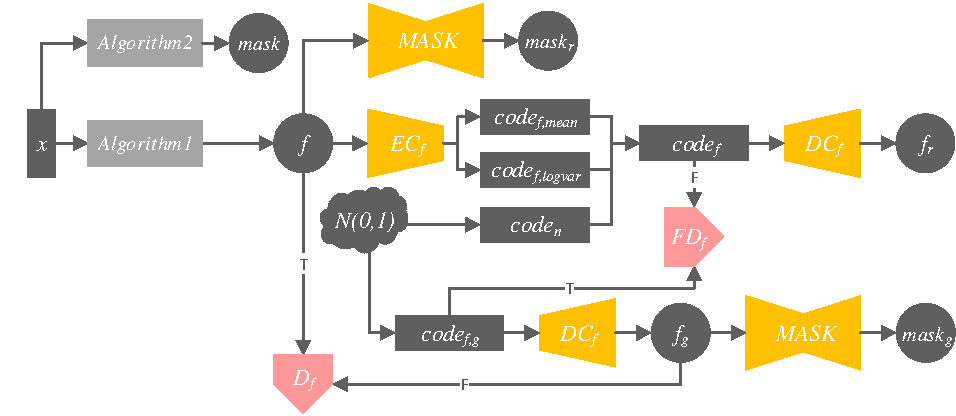
\includegraphics[width=0.98\columnwidth]{figures/feature_train}
	\caption{随机结构特征图的生成训练.Training of Random Structural Feature Map Generation.}
	\label{feature_train}
\end{figure}

为了防止通过结构特征图生成的脑MRI像素区域超出结构特征图的脑轮廓线之外,我们还训练了一个从脑结构特征图获取脑部区域掩膜的生成器$MASK$,该生成器与结构特征图的生成训练进行同步训练。训练时,将真实脑MRI$x$通过掩模提取算法提取得到的掩膜作为训练标签数据,掩膜的提取算法如算法2所示。
In order to prevent the generated brain MRI pixel area from exceeding the brain outline of the structural feature map, we train a generator $MASK$ that acquires the brain area mask from the brain structure feature map. The generator is synchronized with the  training of structural feature map generation. During training, the mask extracted by the real brain MRI$x$ through the mask extraction algorithm (Algorithm~\ref{alg:2}) is used as label data.
\begin{algorithm}
	\caption{Mask Extraction}
	\label{alg:2}
	\begin{algorithmic}[1]
		\State Input a real image $x$, $p$ is expanded pixel value
		\State $mask = 1.0 - ones * (x > 0.)$
		\State $shape = get\_shape(x)$
		\State $mask = resize(mask, size=[shape[1] + p, shape[2] + p])$
		\State $mask = crop\_padding(mask, crop\_length=p, crop\_width=p)$
	\end{algorithmic}  
\end{algorithm}

如图~\ref{feature_train}所示,从标准正态分布解码得到随机结构特征图的具体处理过程如下:
As shown in Fig.~\ref{feature_train}, the specific processing procedure for decoding the random structure feature map from standard normal distribution is as follows:
\begin{itemize}
	\item 从真实MRI$x$中用结构特征提取方法得到结构特征图$f$,用掩模提取算法(算法~\ref{alg:2})生成掩模$mask$;
	The structural feature map $f$ is obtained from real MRI$x$ using the structural feature extraction method, and the mask $mask$ is obtained by the mask extraction algorithm(Algorithm~\ref{alg:2});
	\item 用编码器$EC_f$对结构特征图$f$进行编码获得$code_{f,mean}$及$code_{f,logvar}$,从正态分布$\mathcal{N}(0,1^2)$的获取随机噪声$code_n$,由三个编码求得近似正态分布矩阵$code_f=code_{f,mean}+exp(0.5*code_{f,logvar})*code_n$;
	Encode $f$ with encoder $EC_f$ to get $code_{f,mean}$ and $code_{f,logvar}$, get a random noise $code_n$ from multidimensional normal distribution $\mathcal{N}(0,1^2)$ , the approximate normal distribution matrix is obtained from three codes $code_f=code_{f,mean}+exp(0.5*code_{f,logvar})*code_n$ ;
	\item 用解码器$DC_f$对$code_f$解码得到重建的结构特征图$f_r$;
	Decode $code_f$ with decoder $DC_f$ to obtain the reconstructed structural feature map $f_r$;
	\item 用掩模生成器$MASK$从$f$提取得到掩模$mask_r$;
	Use mask generator $MASK$ to extract mask $mask_r$ from $f$;
	\item 随机生成符合正态分布$\mathcal{N}(0,1^2)$的矩阵$code_{f,g}$;
	Randomly generate a matrix $code_{f,g}$ that obeys normal distribution $\mathcal{N}(0,1^2)$;
	\item 用解码器$DC_f$对$code_{f,g}$解码得到生成的随机结构特征图$f_g$;
	Decode $code_{f,g}$ with decoder $DC_f$ to get the generated random structure feature map $f_g$;
	\item 用掩模生成器$MASK$对$f_g$提取得到掩模$mask_g$;
	Use mask generator $MASK$ to extract mask $mask_g$ from $f$;
	\item 结构特征图鉴别器$D_f$分别对$f$和$f_g$进行鉴别,将前者鉴别为真,后者鉴别为假;
	Structural feature discriminator $D_f$ identifies $f$ and $f_g$ respectively, identifying the former as true and the latter as false;
	\item 编码分布鉴别器$FD_f$分别对$code_f$和$code_{f,g}$进行鉴别,将前者鉴别为假,后者鉴别为真。
	Code distribution discriminator $FD_f$ discriminates between $code_f$ and $code_{f,g}$, respectively, identifying the former as false and the latter as true.
\end{itemize}

训练过程中的各项损失函数如下,其中,$\omega_{i,j}$为各损失项的权重:
In training, we perform adversarial training through discriminator $D_f$ to make the structural feature map decoded by decoder more realistic. In addition, the adversarial training is performed by the feature discriminator $FD_f$, so that encoder $EC_f$ can encode structural feature map $f$ to standard normal distribution. The complete loss items are as follows, where $\omega_{i,j}$ is the weight of each loss item: 
\begin{itemize}
	\item \textbf{编码鉴别器损失Discriminator Loss of Code Distribution } 
	\begin{center}
		$loss_{FD_f}=\Vert{FD_f(code_{f,g})-1}\Vert_{2}^{2}+\Vert{FD_f(code_f)}\Vert_{2}^{2}$
	\end{center}
	
	\item \textbf{结构特征图鉴别器损失Discriminator Loss of Structural Feature Map} 
	\begin{center}
		$loss_{D_f}=\Vert{D_f(f)-1}\Vert_{2}^{2}+\Vert{D_f(f_g )}\Vert_{2}^{2}$
	\end{center}
	
	\item \textbf{对抗性损失Adversarial Loss} 
	\begin{center}
		$loss_{G_f}=\Vert{FD_f(code_f)-1}\Vert_{2}^{2}+\Vert{D_f(f_g)-1}\Vert_{2}^{2}$
	\end{center}
	
	\item \textbf{结构特征编码的分布监督损失Supervised Loss of Structural Feature Code Distribution} 
	\begin{center}
		$loss_{normal}=\Vert{mean(code_{f,mean})}\Vert_{2}^{2}+ \Vert{mean(exp(0.5*code_{f,logvar}))-1}\Vert_{2}^{2}$
	\end{center}
	其中,$mean()$函数为均值函数。
	where $mean()$ is a mean function.
	
	\item \textbf{结构特征图及掩模的自监督损失Self-supervised Loss of Structural Feature Map and Mask} 
	\begin{center}
		$loss_{sv}=\Vert{f-f_r}\Vert_{2}^{2}+\Vert{f_r*mask}\Vert_{2}^{2}$
	\end{center}
	
	\item \textbf{掩膜生成器损失Mask Generator Loss}
	\begin{center}
		$loss_{mask}=\Vert{mask-mask_r }\Vert_{2}^{2}+\Vert{f*mask_r}\Vert_{2}^{2}+\Vert{f_r*mask_r}\Vert_{2}^{2}+\Vert{f_g*mask_g}\Vert_{2}^{2}$
	\end{center}
\end{itemize}

\subsection{真实MRI重建和转换训练Real MRI reconstruction and translation training}
我们在真实的MRI上进行MRI的重建和转换训练,用到了一套MRI编码器、MRI解码器和MRI鉴别器,以及一组病灶标签生成组件。这个训练过程中的全部组件会在后面的多模态MRI生成训练部分中介绍对它们进行的其他训练,并且本节的训练过程与多模态MRI生成训练是同步进行的。我们通过在真实数据上的同步MRI重建和转换训练来约束各个组件在多模态MRI生成的过程中完成我们指定的任务。此外我们还通过一个编码鉴别器来对两个训练过程进行一致性指导。鉴别器训练过程如图~\ref{train_D}所示。
We perform MRI reconstruction and translation training on real MRI, using a set of MRI encoder, MRI decoder and MRI discriminator, as well as a set of lesion label generation components. All of the components of this training process will be described in the subsequent multimodal MRI generation training section, and the training process in this section is synchronized with the multimodal MRI generation training. We constrain each component to complete our assigned tasks during multimodal MRI generation by synchronous MRI reconstruction and translation training on real data. In addition, we also use a code discriminator to guide the consistency of the two training processes. The discriminator training process is shown in Fig.~\ref{train_D}

\begin{figure}
	\centering
	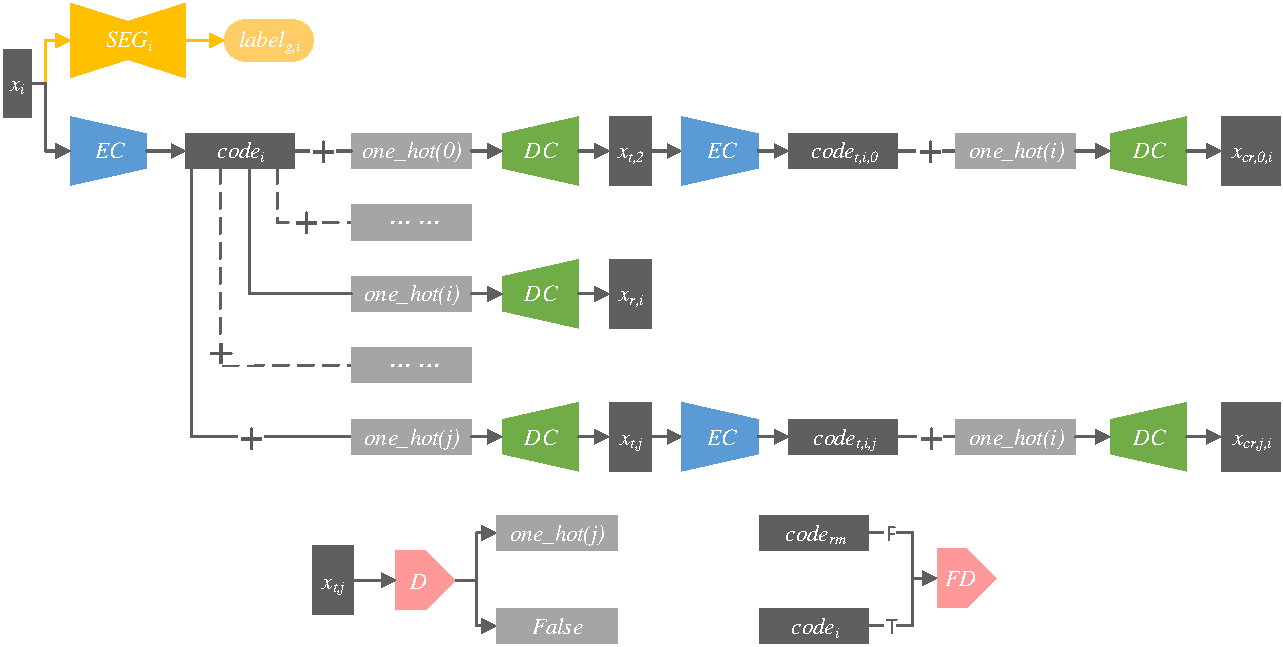
\includegraphics[width=0.98\columnwidth]{figures/trans_train}
	\caption{辅助的模态重建和模态转换训练.Auxiliary modality reconstruction and modality translation training.}
	\label{trans_train}
\end{figure}

如图~\ref{trans_train}所示,MRI重建和转换时,编码器将模态$i$的真实MRI$x_i$编码得到语义特征图$code_{i}$,然后我们将其与不同的条件向量堆叠,通过解码器解码出全部的模态。循环重建时,我们对所得到的转换图采用编码器全部进行再编码,将全部再编码得到的语义特征图均与模态$i$的条件向量进行连接,最后再用解码器全部解码得到循环重建的$x_{rc,j,i}$。MRI重建的循环重建都是自监督训练。在上述过程中,我们以原始输入模态$x_i$对应的病灶标签$l_i$作为病灶生成训练的监督标签,对$x_i$用病灶标签生成组件得到$l_{r,i}$。
As shown in Fig.~\ref{trans_train}, when the MRI is reconstructed and translated, the encoder encodes the real MRI $x_i$ of modality $i$ to obtain the semantic feature map $code_{i}$, then we connect it to different conditional vectors and decode all the modalities through the decoder. In cycle-reconstruction, we use encoder to re-encode all the obtained translation images, connect all the re-encoded semantic feature maps with the conditional vector of modality $i$, and finally decode them by decoder to get cycle-reconstruction image $x_{rc,j,i}$. 【】
In the above process, we use the lesion label $l_i$ of the original input modality $x_i$ as supervised label for the lesion generation training, and use lesion label generation components for $x_i$ to get $l_{r,i}$.

我们的鉴别器组件独立更新,其他组件通过一个优化器更新训练,损失项包括鉴别器提供的对抗性损失、MRI重建自监督损失、MRI循环重建自监督损失、MRI循环重建一致性损失、语义一致性损失、病灶生成监督损失。详细损失如下,其中$x_{r,i}$表示模态$i$重建得到的MRI,$x_{t,j,i}$指由模态$j$转换生成的模态$i$的MRI,$d_{t,j,i}$和$c_{t,j,i}$分别为鉴别器对$x_{t,i,j}$的真假鉴别和类别鉴别结果,$x_{cr,j,i}$表示模态$i$转换为模态$j$再转换回模态$i$的MRI;$code_i$表示编$x_i$编码器编码后得到的语义特征图,$code_{t,i,j}$表示$x_i$转换生成的模态$j$的MRI再经过编码器编码后得到的语义特征图;$l_i$表示$x_i$的真实病灶标签,$l_{r,i}$表示$x_i$经过病灶标签生成组件生成的病灶标签:
Our discriminator components are updated independently, and other components are updated through an optimizer. The loss items include the adversarial loss and category guidance loss provided by discriminator, self-supervised loss of MRI reconstruction, self-supervised loss of MRI cycle-reconstruction, consistency loss of MRI cycle-reconstruction, semantic consistency loss, and supervised loss of lesion generation. 

The detailed losses are as follows, where $x_{r,i}$ represents the MRI reconstruct from modality $i$, and $x_{t,j,i}$ refers to MRI of modality $i$ translated by modality $j$. $d_{t, j, i}$ and $c_{t, j, i}$ are the true/false discrimination and category discrimination results of the discriminator for $x_{t, i, j}$, $x_{cr,j,i}$ represents MRI that translate from modality $i$ to modality $j$ then translate back to modality $i$; $code_i$ represents the semantic feature map obtained from $x_i$ by encoder, $code_{t,i,j}$ represents the semantic feature map obtained from $x_{t,i,j}$ by encoder; $l_i$ represents the real lesion label of $x_i$, $l_{r,i}$ represents the lesion label generated by lesion label generation components from $x_i$ :

\begin{itemize}
	\item \textbf{鉴别器损失discriminator loss}
	\begin{center}
		$loss_{D,assist}=\sum\limits_{j=0,j\neq i}\sum\limits_{i=0}(\Vert{d_{t,j,i}}\Vert_{2}^{2}+\Vert{c_{t,j,i}-i}\Vert_{2}^{2})$
	\end{center}
	
	\item \textbf{对抗性损失和类别指导损失adversarial loss and category guidance loss}
	\begin{center}
		$loss_{G,assist}=\sum\limits_{j=0,j\neq i}\sum\limits_{i=0}(\Vert{d_{t,j,i}-1}\Vert_{2}^{2}+\Vert{c_{t,j,i}-i}\Vert_{2}^{2})$
	\end{center}
	
	\item \textbf{MRI重建自监督损失self-supervised loss of MRI reconstruction}
	\begin{center}
		$loss_{sv}=\sum\limits_{i=0}(\Vert{x_i-x_{r,i}}\Vert_{2}^{2})$
	\end{center}
	
	\item \textbf{MRI循环重建自监督损失self-supervised loss of MRI cycle-reconstruction}
	
	\begin{center}
		$loss_{cycle}=\sum\limits_{j=0,j\neq i}\sum\limits_{i=0}(\Vert{x_i-x_{cr,j,i}}\Vert_{2}^{2})$
	\end{center}
	
	\item \textbf{MRI循环重建一致性损失consistency loss of MRI cycle-reconstruction}
	\begin{center}
		$loss_{cycle,consistency}=\sum\limits_{k=0,k\neq j,k\neq i}\sum\limits_{j=0,j\neq i}\sum\limits_{i=0}(\Vert{x_{cr,j,i}-x_{cr,k,i}}\Vert_{2}^{2})$
	\end{center}
	
	\item \textbf{语义一致性损失semantic consistency loss}
	\begin{center}
		$loss_{code,consistency}=\sum\limits_{j=0,j\neq i}\sum\limits_{i=0}(\Vert{code_i-code_{t,i,j}}\Vert_{2}^{2})$
	\end{center}
	
	\item \textbf{病灶生成监督损失supervised loss of lesion generation}
	\begin{center}
		$loss_{sv,l}=\sum\limits_{i=0}\Vert{label_i-label_{r,i}}\Vert_{2}^{2}$
	\end{center}
	
\end{itemize}

\subsection{结构特征图与病灶分割标签的融合Fusion of structural feature maps and lesion segmentation labels}

结构特征图与病灶分割标签融合时,我们先从随机标准正态分布矩阵生成结构特征图$f_g$,再随机选择合适的病灶分割标签$label$,然后再将包含$n$个类别的病灶分割标签转为$n$个通道的独热矩阵$onehot_l$,每个通道对应一个分割类别,每个通道内的像素值为0或1,与对应类别分割位置相同的区域像素值为1其余部分为0,这样各个1像素区域与分割标签图中的各个分割区域就是配准的。接下来,我们将$onehot_l$的每个通道与$f_g$按位求取加权和,就得到一个新的融合了$f_g$和$label$信息的矩阵。
When the structural feature map is fused with the lesion segmentation label, we first generate structural feature map $f_g$ from random standard normal distribution matrix, then randomly select the appropriate lesion segmentation label $label$, and then the lesion segmentation label containing $n$ categories is converted into a one-hot matrix $onehot_l$ of $n$ channels, and each channel corresponds to a segmentation category, the pixel value in each channel is 0 or 1. The pixel value of the same area as the corresponding category segmentation position is 1 and the rest is 0, so that each 1 pixel area is registered with each segmentation area in the segmentation label. Next, we calculate the weighted sum of each channel of $onehot_l$ with $f_g$, and get a new matrix that fuses the information of $f_g$ and $label$.

如果结构特征图$f'$是从随机MRI$x$中提取的,那么提取出的结构特征有可能包含肿瘤结构信息,会对随机标签$l$中的肿瘤信息产生干扰而影响融合后生成的MRI,所以$f'$需要在与随机标签$label$融合前消除肿瘤信息,得到无肿瘤信息的结构特征图$f$,使生成图像的肿瘤信息只来源于标签$label$。我们对$x$的分割标签$label_x$通过算法~\ref{alg:2}生成无边界扩充的分割掩膜$mask_{l,x}$,则$f=mask_{l,x}\times f'$。
If the structural feature map $f'$ is extracted from the random MRI $x$, then the extracted structural features may contain tumor structure information, which may interfere with the tumor information in random label $l$ and affect the fusion generation MRI, so $f'$ needs to eliminate the tumor information before fusing with the random label $label$, and get the structural feature map $f$ without tumor information, so that the tumor information of the generated image is only derived from the label $label$. We generate a  mask without boundary expansion $mask_{l,x}$ for segmentation label $label_x$ of $x$ by the Algorithm~\ref{alg:2}, then we have $f=mask_{l,x}\times f'$.

由于随机选择的病灶的位置上可能出现在结构特征图的脑部轮廓之外,因此我们选取标签图时需要用算法~\ref{alg:2}获取结构特征图的脑部区域掩膜$mask$,若$mask$与选取的$label$求积后为0,则说明肿瘤标签像素在$mask$的脑轮廓内部,可以采用,否则需要重新选取$label$。
Since the location of the randomly selected lesion may appear outside the brain contour of structural feature map, we need to use the Algorithm~\ref{alg:2} to obtain the brain region mask $mask$ of the structural feature map. If the product of $mask$ and the selected $label$ is 0, then the tumor label pixel is inside the brain contour of $mask$, which can be adopted, otherwise the $label$ needs to be re-selected.

\subsection{多模态MRI生成训练Multimodal MRI generation training}
\begin{figure}
	\centering
	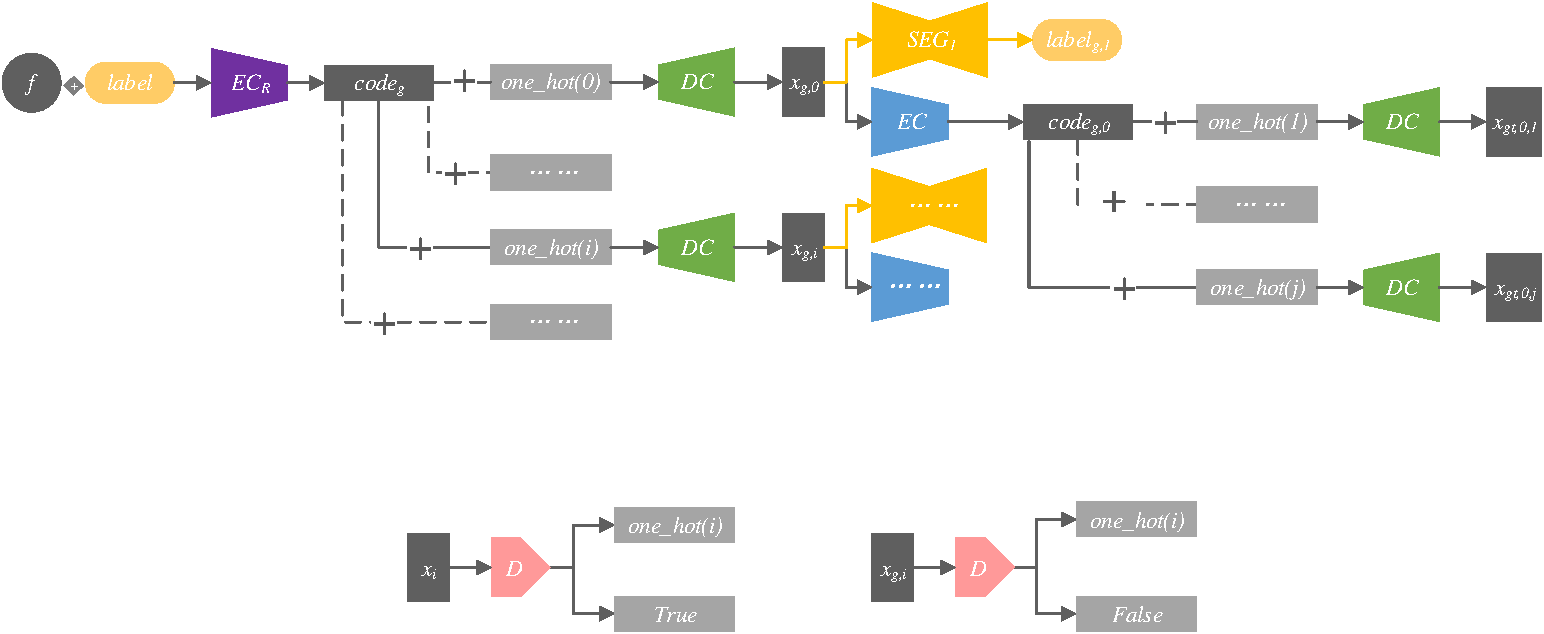
\includegraphics[width=0.98\columnwidth]{figures/mm_mri_generate}
	\caption{多模态MRI生成.generation of Multimodal MRI.}
	\label{mm_mri_generate}
\end{figure}

\begin{figure}
	\centering
	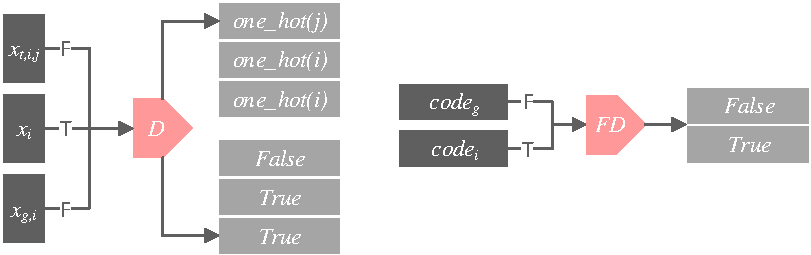
\includegraphics[width=0.8\columnwidth]{figures/D}
	\caption{真实MRI重建和转换训练和多模态MRI生成训练过程中的鉴别器训练. reconstruction and translation training of real MRI and discriminator training during multimodal MRI generation training.}
	\label{train_D}
\end{figure}

我们通过算法~\ref{alg:1}从真实MRI提取结构特征图$f$,并随机选择真实的病灶标签$label$,通过前述结构特征图与病灶分割标签的方法进行融合。结构特征图与分割标签图的信息融合图包含了目标部位的基本解剖结构信息和病灶信息,从该图生成多模态图比直接从随机噪声生成多模态MRI更易训练,生成的MRI更加合理和逼真。多模态MRI生成过程如图~\ref{mm_mri_generate}所示,首先,我们使用一个单独的融合图编码器对信息融合图进行编码得到语义特征图,语义特征图与不同的条件向量堆叠后通过一个MRI解码器解码,得到不同模态的合成图。我们通过一个MRI鉴别器提供的对抗性损失和类别指导损失来使得生成的各个模态的合成图逼近于真实的MRI。各个模态的合成图再通过一个MRI编码器得到语义特征图,然后这些语义特征图与不同的条件向量堆叠后通过MRI解码器解码就实现了模态的转换,我们通过损失对所有语义特征图和转换图进行一致性约束,以此保证了生成的多模态MRI的互相配准。此外,我们使用一组病灶标签生成组件从各合成MRI中分割还原出肿瘤病灶分割标签,确保生成的多模态影像根据输入病灶标签生成了对应的病灶内容。
We extract the structural feature map $f$ from the real MRI by the Algorithm~\ref{alg:1}, and randomly select the real lesion label $label$, and merge with the lesion segmentation label by the above fusion method. The fusion map contains basic anatomical information and lesion information of the target site. The multimodal MRI generated from the fusion map is easier to train than the multimodal MRI generated directly from random noise, and the generated MRI is more reasonable and realistic. The multimodal MRI generation process is shown in Fig.~\ref{mm_mri_generate}. First, we use a fusion map encoder to encode fusion map to obtain the semantic feature map. The semantic feature map is stacked with different conditional vectors and decodes by MRI decoder to obtains synthesis image of different modalities. We use adversarial loss and category guidance loss provided by MRI discriminator to constrain synthesis image to approximate real MRI. And images of each modalities are then encoded by MRI encoder to obtain semantic feature maps. These semantic feature maps are stacked with different conditional vectors and decoded by MRI decoder to realize the modal translation. We constrain the consistency of all semantic feature maps and translation images by loss, thus ensuring the mutual registration of generated multimodal MRI. In addition, we used a set of lesion label generation components to segment the tumor lesion segmentation labels from each synthetic MRI to ensure that the generated multimodal images have generated corresponding lesion content based on the input lesion label.

我们的鉴别器组件独立更新;病灶标签生成组件仅在前面章节中的真实MRI重建和转换训练中采用真实数据训练更新,在本节合成训练过程中病灶标签生成组件仅用于为MRI生成组件提供病灶生成指导损失;其他的组件通过一个优化器更新训练。多模态MRI生成过程的具体损失函数如下,其中$d_{i}$和$c_{i}$为鉴别器$D(x_i)$的真假鉴别输出和类别鉴别输出,$d_{g,i}$,$c_{g,i}$为$D(x_{g,i})$的输出;$x_{g,i}$为模态$i$的合成图,$x_{gt,j,i}$为模态$j$的合成图转换生成的模态$i$的转换图;$code_g$为输入信息编码后的语义特征图,$code_{g,i}$为$x_i$编码后的语义特征图;$l$为输入的标签图,$l_{g,i}$为$x_{g,i}$通过病灶标签生成组件得到的标签图;$f$为输入的结构特征图,$f_{g,i}$为从$x_{g,i}$通过算法~\ref{alg:1}提取得到的结构特征图:
Our discriminator components are updated independently. The lesion label generation component is only trained and updated using real data in reconstruction and translation training, and is used in this section only to provide lesion generation guidance loss for MRI generation components. Other components are updated through an optimizer.

The specific loss items of the multimodal MRI generation process are as follows, where $d_{i}$ and $c_{i}$ are the rue/false discrimination and category discrimination of the discriminator $D(x_i)$, $d_{g, i}$,$c_{g,i}$ is the output of $D(x_{g,i})$; $x_{g,i}$ is the synthetic image of modality $i$, $x_{gt,j,i}$ is the translation image of the modality $i$ translated by synthetic image of modality $j$; $code_g$ is the semantic feature map obtained by fusion map encoder$EC_R$, $code_{g,i}$ is the semantic feature map encoded from $x_i$; $l$ is the input label, $l_{g,i}$ is the label obtained by lesion label generation component from $x_{g,i}$; $f$ is the input structural feature map, $f_{g,i}$ is the structural feature map extracted from $x_{g,i}$ by Algorithm~\ref{alg:1}
\begin{itemize}
	\item \textbf{鉴别器真假鉴别损失 true/false Discrimination loss of Discriminator}
	\begin{center}
		$loss_{D}=\sum\limits_{i=0}(\Vert{d_{i}-1}\Vert_{2}^{2}+\Vert{d_{g,i}}\Vert_{2}^{2})$
	\end{center}

	\item \textbf{鉴别器模态鉴别损失 modality Discrimination loss of Discriminator}
	\begin{center}
	$loss_{D,class}=\sum\limits_{i=0}(\Vert{c_{i}-i}\Vert_{2}^{2}+\Vert{c_{g,i}-i}\Vert_{2}^{2})$
	\end{center}

	\item \textbf{对抗性损失adversarial loss}
	\begin{center}
		$loss_{G}=\sum\limits_{i=0}(\Vert{d_{g,i}-1}\Vert_{2}^{2})$
	\end{center}
	
	\item \textbf{模态类别指导损失Modality category guidance loss}
	\begin{center}
		$loss_{G,class}=\sum\limits_{i=0}(\Vert{c_{g,i}-i}\Vert_{2}^{2})$
	\end{center}
	
	\item \textbf{输入的结构特征图的重建自监督损失Reconstruction self-supervised loss of input structural feature map}
	\begin{center}
		$loss_{sv,f}=\sum\limits_{i=0}(\Vert{f-f_{g,i}}\Vert_{2}^{2})$
	\end{center}
	
	\item \textbf{病灶标签生成监督损失supervised loss of Lesion label generation }
	\begin{center}
		$loss_{sv,l}=\sum\limits_{i=0}(\Vert{label-label_{g,i}}\Vert_{2}^{2})$
	\end{center}
	
	\item \textbf{MRI配准监督损失supervision loss of MRI registration}
	\begin{center}
		$loss_{trans}=\sum\limits_{j=0,j\neq i}\sum\limits_{i=0}(\Vert{x_{g,i}-x_{gt,j,i}}\Vert_{2}^{2})$
	\end{center}
	
	\item \textbf{语义一致性损失semantic consistency loss}
	\begin{center}
		$loss_{trans,code}=\Vert{code_g-code_{g,i}}\Vert_{2}^{2}+\sum\limits_{j=0,j\neq i}\sum\limits_{i=0}(\Vert{code_{g,i}-code_{g,j}}\Vert_{2}^{2})$
	\end{center}
	
\end{itemize}

\subsection{病灶标签生成指导方案Lesion label generation guidance method}
\label{label gen methods}
我们设计了如下三种病灶标签生成组件来提供多模态MRI生成训练中病灶生成的指导损失:
We design the following three lesion label generation components to provide guidance loss for lesion generation in multimodal MRI generation training:
\begin{itemize}
	\item \textbf{单分割器方案Single segmentor} 
	每个模态由一个共同的完整的分割器从合成的MRI还原得到各自的病灶标签。
	Each modality is segmented from synthetic MRI by a common complete segmentor to obtain the respective lesion label.
	\item \textbf{单病灶编码器+多病灶解码器方案Single lesion encoder + multiple lesion decoders} 
	不同模态的分割器由一个共同的病灶编码器与不同的病灶解码器组合得到.
	Different modality segmentors are combined by a common lesion encoder and different lesion decoders. 
	\item \textbf{多分割器方案multiple segmentors} 
	每个模态由一个独立的完整的分割器从合成的MRI还原得到各自的病灶标签。
	Each modality is segmented from synthetic MRI by a separate complete segmentor to obtain the respective lesion label.
\end{itemize}
上述三种方案的损失函数与前文所述损失函数一致,三种方案中的各个组件均只使用真实MRI重建和转换训练中的病灶生成监督损失进行训练。
The loss item of the above three schemes is consistent with the loss item described above, and each component of the three methods is only trained using supervised loss of lesion label generation in real MRI reconstruction and translation training.

\subsection{构建合成数据集construction of synthetic datasets}
\label{make dataset}
如图所示,我们通过训练好的结构特征图解码器即可从随机生成的正太分布矩阵生成任意数量的结构特征图。然后,我们对原始的标签集进行了随机的缩放、旋转、平移、翻转等改变得到随机病灶标签集。我们再将随机生成的结构特征图和从随机病灶标签集中随机选择的病灶标签融合,同样地,我们通过掩膜生成器$MASK$生成结构特征图的掩膜,可以筛选得到合适的随机病灶标签。最后,我们通过多模态MRI生成组件即可从融合信息图中生成配准的多模态MRI,选取的病灶标签就是生成的多模态MRI的病灶标签。由此,我们可以从随机正态分布矩阵构建带有病灶标签的多模态配准MRI数据集。
As shown in Fig.~\ref{make_data}, we can generate any number of structural feature maps from randomly generated normal distribution matrix through the trained structural feature map decoder. Then, we randomly scaled, rotated, translated, flipped, etc. the original set of labels to get a random lesion label set. We then fuse the randomly generated structural feature map with the randomly selected lesion label from the random lesion label set. Similarly, we can select suitable random lesion labels by obtaining mask from structural feature map through the mask generator $MASK$. Similarly, we can select suitable random lesion labels by obtaining mask from structural feature map through the mask generator $MASK$. Finally, we synthesize registered multimodal MRI from the fusion map by multimodal MRI generation components. And the selected lesion label is the lesion label of the synthetic multimodal MRI. Thus, we can construct a multimodal registration MRI dataset with lesion labels from a random normal distribution matrix.
\begin{figure}
	\centering
	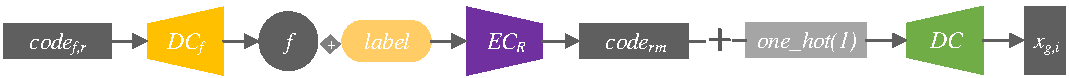
\includegraphics[width=0.98\columnwidth]{figures/make_data}
	\caption{构建合成数据集.construction of synthetic datasets.}
	\label{make_data}
\end{figure}

由于训练时去除肿瘤信息操作的影响,合成的结构特征图中,存在一些质量较差的脑轮廓未闭合结构特征图,我们对此设计了一个结构特征图过滤算法。首先,我们使用生成器生成一张结构特征图和其对应的掩膜,我们先对结构特征图进行高斯模糊\cite{92wink2004denoising},再采用OpenCV【】提供的轮廓查找算法和填充算法获取高斯模糊图所有的闭合轮廓并进行填充,这样我们得到一个采用传统算法的得到的掩膜,最后我们计算两张掩膜的均差(MAE)。若MAE低于我们设定的阈值则说明该结构特征图主要的脑部轮廓较为完整,该特征图可以使用;否则则说明该结构特征图主要的脑部轮廓有残缺,采用传统算法得到的掩膜内部是空心的,与生成器生成的掩膜差异较大,因此,需要重新生成。算法表示如下:
Due to the influence of the operation that removing tumor information during training, there are some structural feature maps with poor quality that brain contour is not closed, so we design a structural feature map filtering algorithm for this. First, we use the generator to generate a structural feature map and its corresponding mask. We perform Gaussian blur\cite{92wink2004denoising} on the structural feature map , and then use the contour search algorithm and filling algorithm provided by OpenCV to obtain all the closed contours of the Gaussian blur image and fill them. So we get a mask by the traditional algorithm, and finally we calculate the Mean Absolute Error (MAE) of the two masks. If the MAE is lower than the threshold we set, the main brain contour of the structural feature map is relatively complete, and the feature map can be used; otherwise, the main brain contour of the structural feature map is defective, the mask obtained by the traditional algorithm is hollow inside and quite different with the mask generated by the generator, so it needs to be regenerated. The algorithm is expressed as follows:
\begin{algorithm}
	\caption{Structural feature map filtering}
	\label{alg:3}
	\begin{algorithmic}[1]
		\State \textbf{function} $GetMaskFromF(img)$
		\State \indent$contours = OpenCV.findContours(img)$
		\State \indent$img =OpenCV.drawContours(img,contours)$
		\State \indent\textbf{return} $img$
		\State \textbf{end function}
		\State
		\State $mae=0.05$
		\State \textbf{do} 
		\State \indent$f, m = Generator()$
		\State \indent$m'= GetMaskFromF(f)$
		\State \textbf{while} $MAE(m',m) <= mae$
	\end{algorithmic}  
\end{algorithm}

从筛选出来的结构特征图和匹配的病灶标签得到的多模态MRI中,同样存在病灶信息生成情况较差的样本。此时,我们通过预先训练好的病灶分割网络对我们的合成MRI数据进行分割,然后将分割结果与输入的病灶标签进行骰子评分评估,可以过滤得到评分高于设定阈值(默认0.95)的样本。
In the multimodal MRI obtained from the selected structural feature map and matched lesion label, there are also samples with poor lesion generation. At this point, we segment our synthetic MRI data through a pre-trained lesion segmentor, the segmentation result is then evaluated with the input lesion label for the dice score, and the sample with the score above the set threshold (default 0.95) can be filtered.

经过多重筛选,我们得到最终的由随机结构特征图、配对的掩膜、随机病灶分割标签、多模态MRI组成的合成数据集。我们要求经过分割过滤后的数据集在使用真实数据训练得到的分割器上能取得0.98以上的骰子分数,然后才能将其用于数据可用性验证实验。
After multiple filtering, we obtain the final synthetic dataset consisting of random structural feature maps, paired masks, random lesion segmentation labels, and multimodal MRI. We require that the segmented and filtered dataset can achieve a score of 0.98 or more on the segmentor trained on real data before it can be used in the data availability verification experiment.

\subsection{病灶分割训练}
\begin{figure}
	\centering
	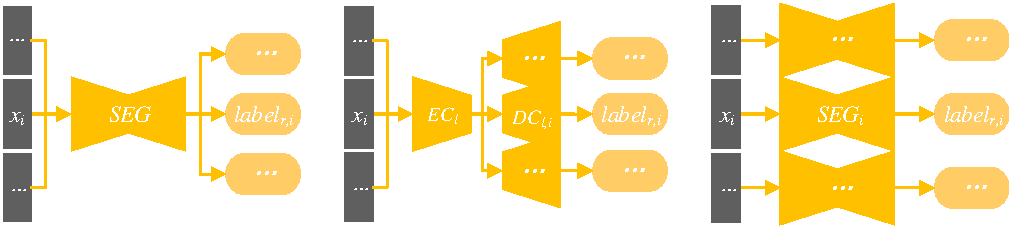
\includegraphics[width=0.45\columnwidth]{figures/segmentation}
	\caption{病灶分割.lesion segmentation.}
	\label{segmentation}
\end{figure}

我们的病灶分割训练过程如图所示,为了验证合成数据中是否生成了与随机输入的病灶标签一致的病灶信息,我们用真实的数据为每个模态单独训练一个独立的病灶分割网络,并在真实数据集中进行分割能力测试。然后使用训练好的分割器对合成数据集中的影像进行分割,将分割结果与输入的病灶标签比对评估,以此检验合成的影像中包含了预期的病灶信息。此外,我们还采用由不同数据量的合成数据和真实数据构建的数据集来训练病灶分割网络,训练充分后再在真实测试数据集上进行分割能力测试,以验证合成数据的可用性。
Our lesion segmentation training process is shown in Fig. In order to verify whether the lesion data in the synthetic data is consistent with the random input lesion label, we use real data to train an independent lesion segmentor for each modality, and perform segmentation ability test on real datasets. The trained segmenter is then used to segment the image in the synthetic dataset, and the segmentation result is compared with the input lesion label to verify that the synthetic image contains the expected lesion information. In addition, we also use a data set constructed from synthetic data and real data of different data volumes to train the lesion segmentor. After training, the segmentation ability test is performed on real test dataset to verify the availability of  synthetic data.

分割训练的损失函数如下,其中$label_{r,i}$表示$x_i$经过病灶分割器生成的病灶标签:
The loss item of the segmentation training is as follows, where $label_{r,i}$ represents lesion label generated by the lesion segmentor from $x_i$
\begin{center}
		$loss_{l}=\sum\limits_{i=0}\Vert{label_i-label_{r,i}}\Vert_{2}^{2}$
\end{center}


\section{实验Experiments}

\subsection{BRATS2015数据集BRATS2015 dataset}
我们采用了公开的BRATS2015\cite{91menze:hal-00935640}数据集进行实验,该数据集包含已配准的T1、T2、T1c、Flair四个模态,训练集每个模态有274张3D MRI,大小为155$\times$240$\times$240,同时配有274张相同尺寸的肿瘤分割标签。我们将样本按9:1划分训练集和测试集,取每张3D MRI第55-105间的50个slice构建2D的数据集。在数据预处理阶段,我们将每张图进行了标准化。
We use the open dataset BRATS2015 for experiments, which has four registered modalities of T1/T2/T1c/Flair. The training dataset contains 274 3D MRIs per modality, with the size of 155$\times$240$\times$240, and 274 tumor segmentation labels of the same size. We divide the sample into a training set and a testing set by 9:1, and construct a 2D data set from 50 slices of each 55-105 of the 3D MRI. In data preprocessing, we standardized each image.

\subsection{BRATS合成数据集BRATS synthetic dataset}
我们采用~\ref{make dataset}中的方法构建了一个配准的包含T1、T2、T1c、Flair四个模态的具有肿瘤标签的合成数据集。合成数据集样本的尺寸与BRATS2015数据集一致,但样本的多少可以根据实验需要进行任意数量的合成。
We constructed a registered synthetic dataset with tumor labels containing four modalities of T1, T2, T1c, and Flair using the method in ~\ref{make dataset}. The size of the synthetic dataset sample is consistent with the BRATS2015 dataset, but the number of samples can be any number according to the needs of the experiment.

\subsection{BRATS增强数据集BRATS Enhanced dataset}
我们对原始的BRATS2015数据集进行了随机的缩放、旋转、平移、翻转等改变,得到增强数据。增强数据集样本的尺寸与BRATS2015数据集一致,但样本的多少可以根据实验需要进行任意数量的生产。
We performed random scaling, rotation, translation, flipping, etc. on the original BRATS2015 dataset to obtain enhanced data. The size of the enhanced dataset sample is consistent with the BRATS2015 dataset, but the number of samples can be any number according to the needs of the experiment.

\subsection{训练设置Training settings}
每项实验的迭代次数与BRATS2015训练数据集的100个epoch相等;基础学习率分别为1e-4,无权重衰减;采用优亚当优化器,beta1取0.5;在输入层进行0.1的Dropout;Batch size为1;在生成器中使用均值滤波器的参数进行参数初始化,具体来说,对于一个卷积核尺寸为$[k,k,f]$的卷积层,我们初始化该层的$k\times k\times f$个卷积核参数均为$1/(k\times k\times f)$, ,偏置量为0。我们采用骰子分数\cite{95dice1945measures}和均方差(MSE)\cite{94prasad1990the}进行分割结果的评估,评估结果为2D图像的评估结果的均值,每项实验训练四次保留最佳结果。
The number of iterations of each experiment is equal to 100 epochs of the BRATS2015 training dataset. The learning rate is 1e-4 without weight decay.  we use Adam optimizer with beta1 of 0.5 and perform a Dropout of 0.1 on the input layer, Batch size is 1. In generator components, the mean kernel filter parameter is used to initialize the convolution kernel parameter. Specifically, for a convolutional layer with a convolution kernel size of $[k,k,f]$, we initialize the $k\times k\times f$ convolution kernel parameters of this layer to $1/(k \times k\times f)$, and the bias is 0. In discriminator, we use a random normal initializer with mean of 0 and standard deviation of 0.2, and the bias is 0. We used Dice Score \cite{95dice1945measures} and Mean Square Error (MSE)\cite{94prasad1990the} to evaluate the segmentation results. The evaluation results are the average of the evaluation results of the 2D images, and each experiment is trained four times to retain the best results.

\subsection{病灶生成组件各方案对比实验Contrast experiment of each method of lesion generation component}
\label{label gen methods tests}
我们使用在处理后的BRATS2015数据集的训练集对病灶分割网络进行了相同迭代步数的充分训练,然后我们在BRATS2015测试数据集和通过不同病灶生成指导方案得到的未经分割器筛选的的合成数据集上分别进行分割测试,除了测试数据来源的不同外,测试数据的样本量等其他条件完全相同。其中,我们在真实数据上采用的分割方案为章节~\ref{label gen methods}中的多分割器方案,即每个模态各训练一个独立的分割器。
We used the training set of the processed BRATS2015 dataset to fully train the lesion segmentor for the same iteration step, and then we selected the test set of the BRATS2015 dataset and  the unfiltered synthetic dataset by segmentor from different lesion generation component methods. Except for the difference in the source of the test data, other conditions such as the sample size of the test data are identical. Among them, the segmentation method we adopt on the real data is the multiple segmentors method in the section~\ref{label gen methods}, that is, each modality trains a separate segmentor.

\subsection{合成数据可用性验证实验 verification experiment of Synthetic data availability}
如表所示,我们将真实的BRATS2015训练数据与BRATS合成数据进行了不同数量的混合,再用构建的混合数据集进行分割训练,最后再在真实的BRATS2015测试数据上进行模型的分割能力评估,所有实验都进行相同迭代步数的充分训练,除了训练数据源的不同外其他条件完全相同。同时,我们还进行了单独的合成数据的训练、真实数据与通常的数据增强数据的混合训练作为对比。我们设定了随机混合、先真后假、先假后真三种数据混合方式。我们选用实验~\ref{label gen methods tests}中,在合成数据集上表现最好的分割方案来作为验证实验的分割方案。
As shown in the table, we mixed real BRATS2015 training data with BRATS synthetic data in different amounts, then used the mixed data set for segmentation training, and finally evaluated the segmentation ability of the model on real BRATS2015 test data. All experiments were fully trained with the same number of iterations. Except for the difference in the source of the training data, other conditions such as the sample size of the test data are identical. At the same time, as a comparison, we also conduct a separate training of synthetic data, mixed training of real data and normal enhancement data. We set up three data mixing modes: random mixing, real first, and synthetic
first.

\section{结果Results}
\subsection{实验量化结果Quantitative result}

\subsubsection{病灶检测实验结果Lesion segmentation result}
\begin{table}[t]
	\caption{病灶检测实验结果.Lesion segmentation result}\smallskip
	\centering
	\resizebox{.95\columnwidth}{!}{		
		\smallskip\begin{tabular}{llll}		
			\toprule	
			synthetic method&test data type &MSE   &Dice Score \\	
			\midrule		
			-&real 		   				&0.026 &0.915 \\					
			1SEG&synthetic     			&0.053 &0.741 \\			
			1ECL+4DCL&synthetic     	&0.055 &0.808 \\		
			4SEG&synthetic     			&0.043 &0.838 \\
			\bottomrule			
		\end{tabular}	
	}	
	\label{label_test}	
\end{table}

如表~\ref{label_test}所示,我们在BRATS2015训练数据经过相同的迭代步数的充分训练后,在真实的测试数据集上,分割测试结果达到了0.026的MSE和0.915的Dice Score。之后我们使用这个表现优秀的分割网络对我们未经过滤的合成数据进行分割测试,在与真实测试数据集相同数据量的合成数据集上,不同病灶标签生成组件设计方案都取得了较好的分割结果,其中每个模态训练一个独立的分割器的方案取得了最好的结果,Dice Score也达到了0.838。
As shown in the table ~\ref{label_test}, after the BRATS2015 training data is fully trained by the same iteration step, the segmentation test results reach the MSE of 0.026 and the Dice Score of 0.915 on the real test data set. Then we use this excellent segmentor to segment our unfiltered synthetic data. On the synthetic dataset with the same amount of data as the real test dataset, three different lesion label generation component methods have achieved good segmentation results. As a result, the method in which each modality trains a separate segmentor achieves the best results, and the Dice Score also reaches 0.838.

\subsubsection{合成数据可用性验证实验结果Verification experiment results for synthetic data availability}
\begin{table}[t]
	\caption{合成数据可用性验证实验结果.Verification experiment results for synthetic data availability}\smallskip
	\centering
	\resizebox{.95\columnwidth}{!}{
		\smallskip\begin{tabular}{lllllll}
			\toprule
			Num &real data &synthetic data & Enhanced data  & mixing modes  & MSE &Dice Score\\
			\midrule
			1& 15070 & 0  &0 &- &0.026 &0.915 \\
			31& 15070$\times$ 0.5 & 0  &0 &- &0.032 &0.902 \\
			
			2& 0 & 15070  &0 &- &0.205 &0.708 \\
			3& 0 & 15070$\times$ 2  &0 &random mixing &0.206 &0.736 \\
			4& 0 & 15070$\times$ 3  &0 &random mixing &0.205 &0.754 \\
			
			7& 15070$\times$ 0.1 & 15070  &0 &synthetic
			first &0.031 &0.908 \\
			8& 15070$\times$ 0.1 & 15070$\times$ 2  &0 &synthetic
			first &0.028 &0.907 \\
			9& 15070$\times$ 0.1 & 15070$\times$ 3  &0 &synthetic
			first &0.030 &0.907 \\	
			
			13& 15070$\times$ 0.2 & 15070$\times$ 0.8 &0  &random mixing &0.041 &0.850 \\
			12& 15070$\times$ 0.5 & 15070$\times$ 0.5 &0  &random mixing &0.031 &0.904 \\
			14& 15070$\times$ 0.8 & 15070$\times$ 0.2 &0  &random mixing &0.024 &0.935 \\
			
			32& 15070 & 15070$\times$ 0.2 &0  &random mixing &0.025 &0.921 \\
			33& 15070 & 15070$\times$ 0.5 &0  &random mixing &0.023 &0.939 \\
			34& 15070 & 15070$\times$ 0.8 &0  &random mixing &0.026 &0.916 \\
			15& 15070 & 15070 &0            &random mixing &0.027 &0.913 \\
			18& 15070 & 15070$\times$ 2  &0 &random mixing &0.033 &0.901 \\
			19& 15070 & 15070$\times$ 3  &0 &random mixing &0.034 &0.897 \\
			
			35& 15070 &0 & 15070$\times$ 0.2   &random mixing &0.027 &0.911 \\
			36& 15070 &0 & 15070$\times$ 0.5   &random mixing &0.025 &0.927 \\
			37& 15070 &0 & 15070$\times$ 0.8   &random mixing &0.026 &0.920 \\
			22& 15070 &0 & 15070           &random mixing &0.026 &0.915 \\
			23& 15070 &0 & 15070$\times$ 2 &random mixing &0.032 &0.898 \\
			24& 15070 &0 & 15070$\times$ 3 &random mixing &0.036 &0.885 \\
			
			16& 15070 & 15070 &0  &real first &0.195 &0.795 \\
			17& 15070 & 15070 &0  &synthetic
			first &0.021 &0.940 \\
			\bottomrule
		\end{tabular}
	}
	\label{use_test}
\end{table}
如表~\ref{use_test}所示,我们在不同的成分和数量的数据集上都经过训练后再在真实测试集上评估,得到了表中的结果。
实验1在BRATS2015训练数据经过100个epoch的充分训练后,在真实的测试数据集上,分割测试结果达到了0.026的MSE和0.915的Dice Score。
从表中实验2-4单独使用合成数据训练的结果看,合成数据与真实数据的训练结果仍然有一定差距,这说明合成数据不能完全替代真实数据充当训练集。
实验7-9结果表明使用大量合成数据进行预训练,再在少量真实数据上微调能达到和实验1全使用真实数据训练十分接近的结果。这说明合成数据作为预训练数据集非常合适。
实验12-14中一定比例的真实数据与合成数据随机混合,比例不同取得的结果差异很大,当两者比例相近时分割结果与实验1相差不大,合成数据比例偏高时,结果比实验1低,合成数据比例偏低时,能提供模型的泛化能力,取得高于实验1的结果。
实验32-34,15,18-19中进一步尝试在全量的真实数据中添加不同数据量的合成数据,我们发现较少的合成数据能提高模型的泛化能力,起到数据增强的作用,合成数据越多增强效果越好,但当合成数据到达一定比例后再继续增加将取得反效果,此时合成数据越多越使得真实数据的影响力下降。
实验35-37和实验22-24中,我们使用通常的数据增强方法产生的增强数据来与前述合成数据的增强效果进行对比,我们发现在增强数据量与增强效果的变化趋势上,两者是一致的,但两者在具体的增强效果随着增强数据量变化的变化曲线上是有一些差异的。整体来说,在模型对增强数据量的敏感程度上,增强数据更加鲁棒,但合成数据能取得的增强效果的上限比曾强数据要高很多。
在实验16-17中,我们对比实验15,发现与真实数据相同数量的合成数据,作为预训练数据先于真实数据训练时表现最好,作为增强数据与真实数据混合训练时效果居中,作为补充训练数据集在真实数据集之后训练则表现很差。
【TO DO】As shown in table ~\ref{use_test}, we have been trained on data sets with different components and quantities and then evaluated on real test sets to get the results in the table.In experiment 1, after the full training of 100 epochs of BRATS2015 training data, the segmentation test results reached 0.026 MSE and 0.915 Dice Score on the real test data set.According to the training results of experiment 2-4 using synthetic data alone in the table, there is still a certain gap between the training results of the synthetic data and the real data, which indicates that the synthetic data cannot completely replace the real data as the training set.The results of experiment 7-9 show that pre-training with a large amount of synthetic data and fine-tuning on a small amount of real data can achieve a result very close to that of training with real data in experiment 1. This indicates that the synthesized data is very suitable as a pre-training data set.Experiment 12-14 a percentage of the real data and synthetic data random mixing proportion of different result difference is very big, when both scale similar segmentation result with experiment 1 were similar, synthesis of high data rate, the result is lower than the experiment 1, synthetic data rate is low, can provide the generalization ability of the model, obtained is higher than the result of experiment 1.Experiment a further attempt to 32-34, 18th - 19 in the total amount of real data synthesis data of adding different amount of data, we found that fewer synthetic data can improve the generalization ability of the model, have the effect of data enhancement, synthetic data enhancement effect, the better, the more but when synthetic data to increase again after a certain proportion will have the opposite effect, the synthetic data, the more the influence of the real data.Experiment 35 to 37 and 22 to 24, we use the enhancement data generated by a data enhancement method to enhancement effect compared with the synthetic data, we found the data volume increased and enhanced effect on the change tendency of the two is consistent, but the difference in specific enhancement effect as the change of enhanced data volume change curve there are some differences. Overall, in terms of the sensitivity of the model to the amount of enhanced data, the enhanced data is more robust, but the upper limit of the enhancement effect that can be achieved by the composite data is much higher than that of the former strong data.In experiment 16-17, we compared experiment 15 and found that the synthesized data with the same amount of real data had the best performance as pre-training data before real data training, the mixed training effect as enhanced data and real data was in the middle, and the training performance after real data set as supplementary training data was very poor.

总的来说,我们发现当真实数据量较多时,可以使用少量的合成数据作为增强数据混合使用,也可以使用大量的合成数据先进行预训练,再在真实数据集上训练;当真实数据较少时,可以使用大量的合成数据进行预训练,再在少量真实数据上微调,最后能得到和完全真实数据训练相竞争的结果,这点我们与\cite{4shin2018medical}的结论一致;我们不建议完全使用合成数据进行训练,与\cite{4shin2018medical}的结论不同的是我们也不建议使用合成数据进行补充训练。
【TO DO】AsIn general, we find that when the amount of real data is large, a small amount of composite data can be used as mixed enhancement data, or a large amount of composite data can be used for pre-training before training on real data sets. When real data is scarce, large amounts of synthetic data can be used for pre-training, and then fine-tuned on a small amount of real data to obtain results that compete with the training of completely real data. This is consistent with the conclusion of \cite{4shin2018medical}. We do not recommend full use of synthetic data for training, and contrary to the conclusion of \cite{4shin2018medical}, we do not recommend supplementary training using synthetic data either.

\subsection{合成图像展示}
图~\ref{generated_f}展示了我们从随即正态分布矩阵生成的结构特征图示例。图~\ref{generated_mri}中展示了我们从随即正态分布矩阵生成的结构特征图、从结构特征图生成的对应的掩膜、随机选择的病灶分割标签、从结构特征图生成和的病灶分割标签生成的多模态MRI的几个示例。

【TO DO】AsFigure ~\ref{generated_f} shows an example of the structural feature graph we generated from the random normal distribution matrix. In figure ~\ref{generated_mri}, we show several examples of structural feature maps generated from random normal distribution matrices, corresponding masks generated from structural feature maps, randomly selected lesion segmentation labels, and multi-modal MRI generated from structural feature maps and lesion segmentation labels.
\begin{figure}
	\centering
	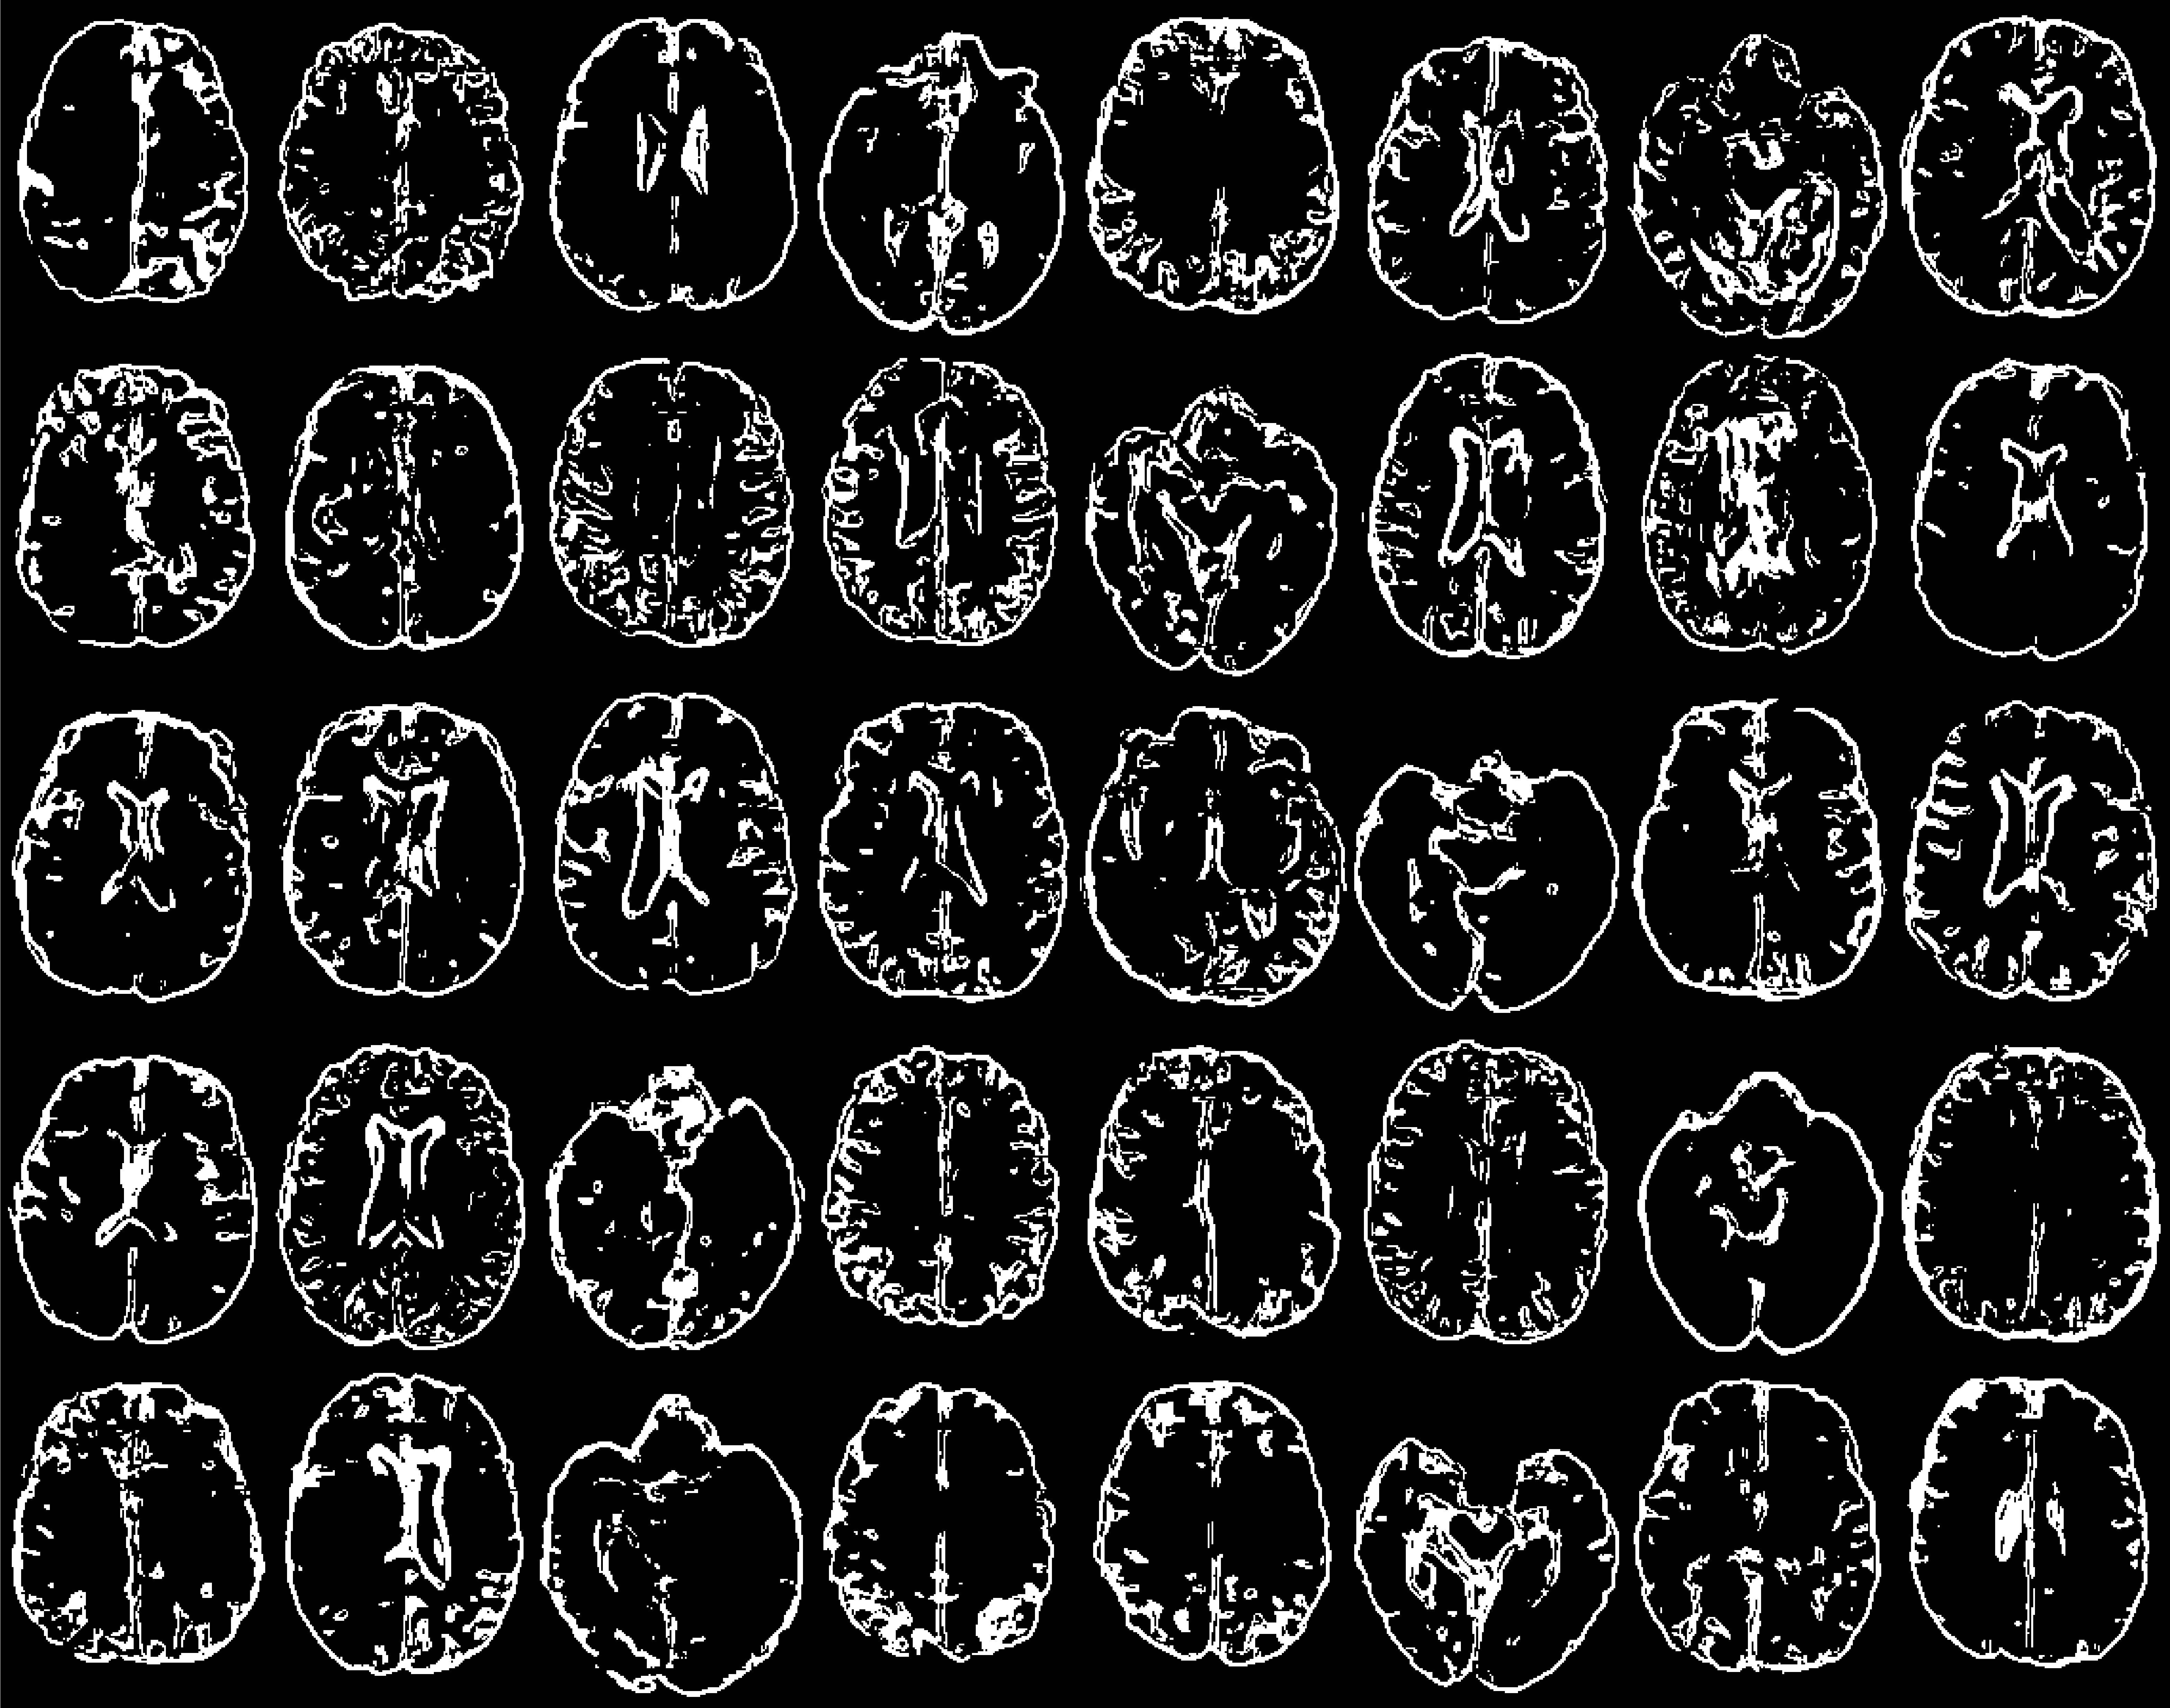
\includegraphics[width=0.98\linewidth]{figures/Fs}
	\caption{合成的结构特征图.}
	\label{generated_f}
\end{figure}

\begin{figure}
	\centering
	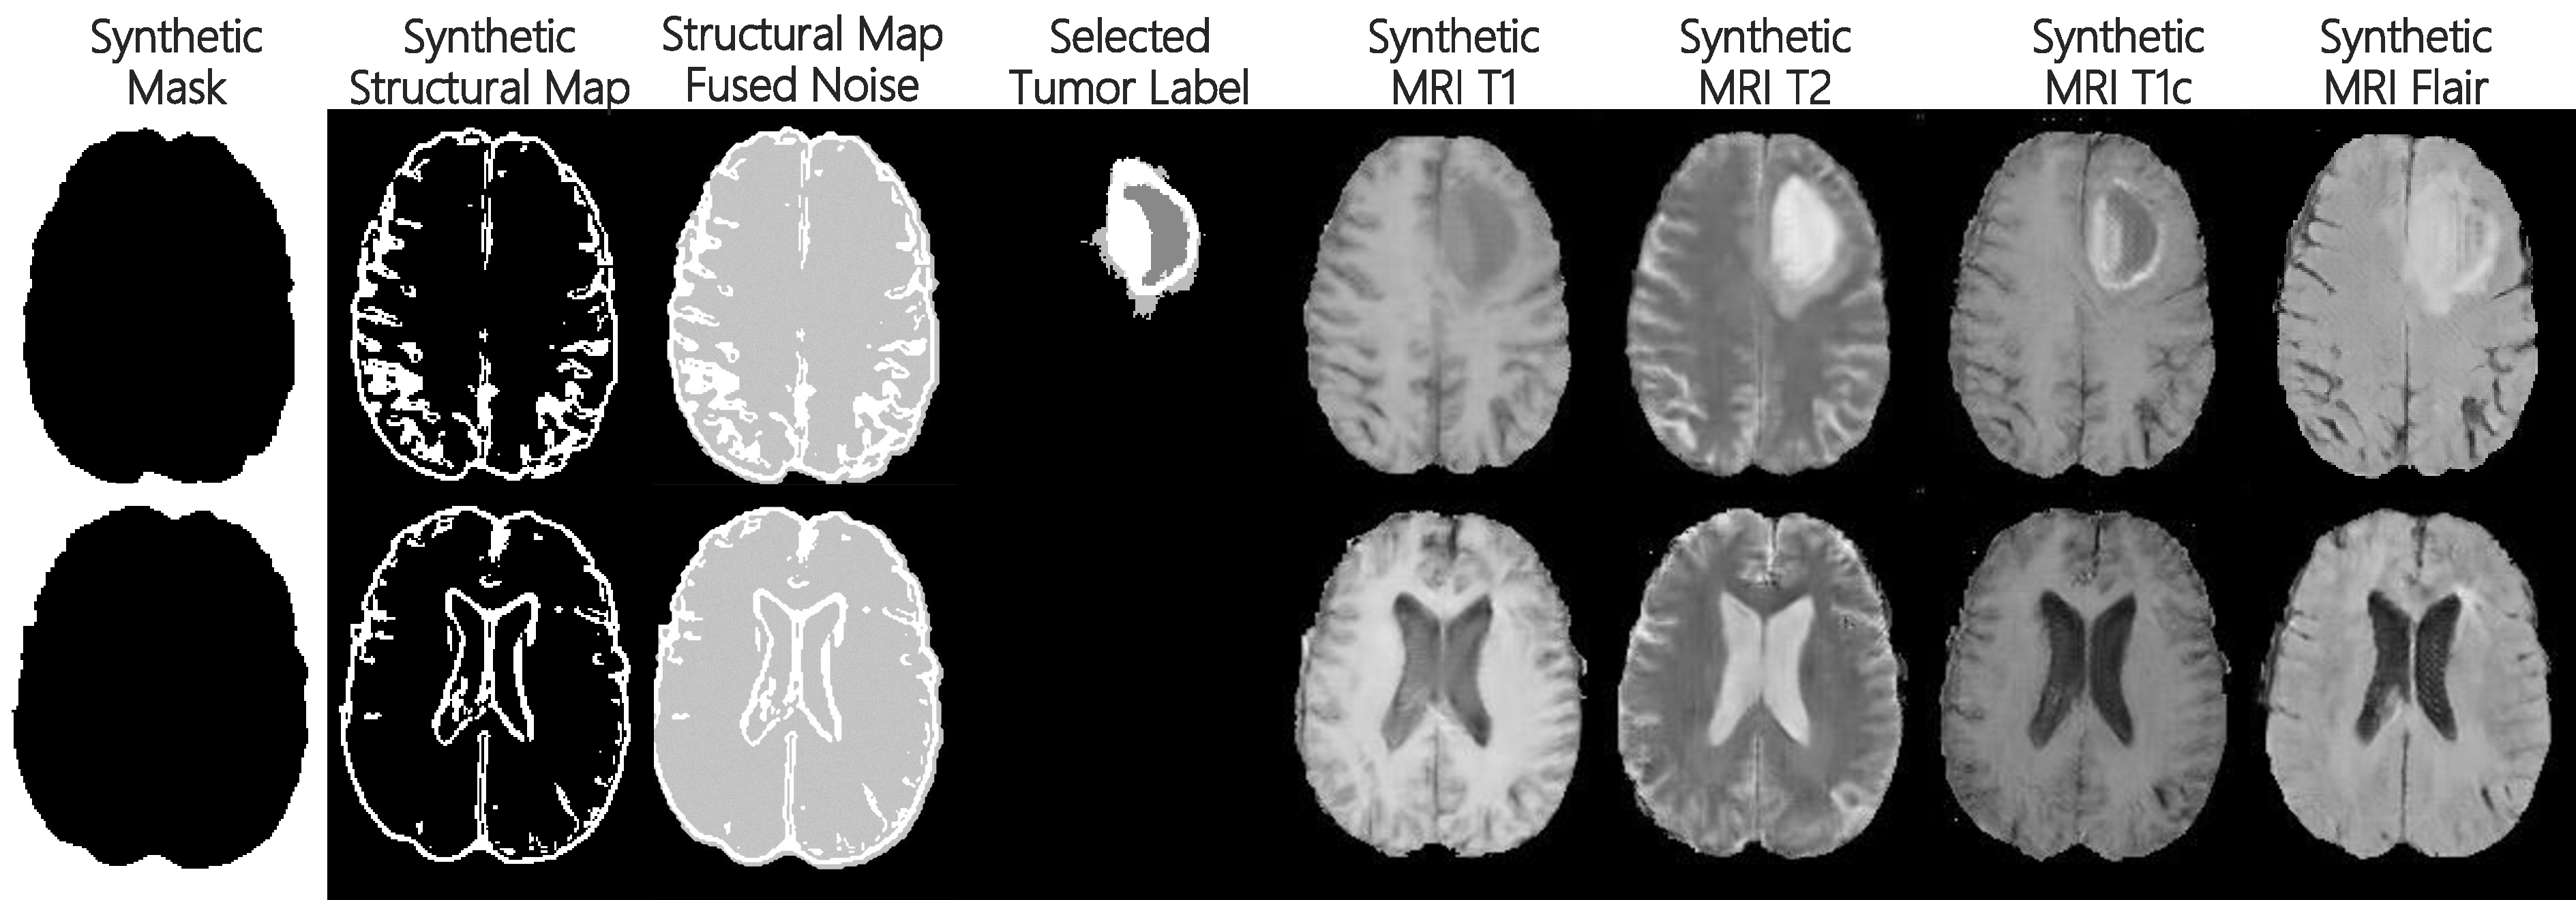
\includegraphics[width=0.98\linewidth]{figures/F_to_MRI}
	\caption{从随机结构特征图和病灶标签生成多模态MRI.}
	\label{generated_mri}
\end{figure}

\section{结论与未来工作}

我们基于条件生成对抗网络,通过无监督的训练,实现了从随机正态分布矩阵生成配准的多模态MRI并能自由添加病灶信息。我们通过病灶分割实验验证了合成的MRI可以作为智能医学影像处理任务的预训练数据或增强数据来使用并能显著提高模型的泛化能力。具体来说,我们的贡献包括以下几点:

Based on the conditional generation antagonism network, we realized the generation of registered multimodal MRI from the random normal distribution matrix through unsupervised training, and could add the lesion information freely. 
We verified through lesion segmentation experiments that synthetic MRI can be used as pre-training data or enhanced data for intelligent medical image processing tasks and can significantly improve the generalization ability of the model.
In this paper, our contributions include the following:
\begin{itemize}
	\item 我们提出了一种从医学影像直接提取解剖结构信息的结构特征图提取方法,无须训练,无需额外数据;
	We propose a structural feature map extraction method to extract anatomical structure information directly from medical images without training or additional label data;
	\item 我们提出了一种从多维正态分布采样生成结构特征图的随机结构特征图生成方法,使结构特征图能便捷地大量生成并具有良好的多样性;
	We propose a random structure feature map generation method to generate structural feature maps from multi-dimensional normal distribution sampling;
	\item 我们实现了从结构特征图及随机选择的病灶标签生成具有对应病灶信息的配准的多模态MRI;
	We realized the generation of registered multimodal MRI with corresponding lesion information from structural feature map and randomly selected lesion labels;
	\item 我们通过多项在合成数据上进行的数据可用性测试,验证了合成数据可以作为智能医学影像处理任务的预训练数据或增强数据来使用。
	We verified that synthetic data can be used as pre-training data or enhanced data for intelligent medical image processing tasks through a number of data usability tests on our synthetic dataset.
	
\end{itemize}

未来,我们将进一步在CT、PET等不同模态,心脏、肺等其他部位,检测、分类等其他病灶处理任务中对我们的方法进行改进。我们将致力于进一步简化训练过程和合成更高质量的医学影像。
In the future, we will further improve our method in CT, PET and other modes, in heart, lung and other parts, in detection, classification and other lesion processing tasks. We are committed to further simplifying the training process and synthesizing higher quality medical images.	

\section{ Acknowledgments}

感谢NSCCGZ提供的计算支持。
Thanks for the computing support provided by NSCCGZ.


\bibliography{refer}
\bibliographystyle{aaai}

\end{document}
